
\documentclass{article} % For LaTeX2e
\usepackage{iclr_template/iclr2025_conference,times}

% Optional math commands from https://github.com/goodfeli/dlbook_notation.
%%%%% NEW MATH DEFINITIONS %%%%%

\usepackage{amsmath,amsfonts,bm}

% Mark sections of captions for referring to divisions of figures
\newcommand{\figleft}{{\em (Left)}}
\newcommand{\figcenter}{{\em (Center)}}
\newcommand{\figright}{{\em (Right)}}
\newcommand{\figtop}{{\em (Top)}}
\newcommand{\figbottom}{{\em (Bottom)}}
\newcommand{\captiona}{{\em (a)}}
\newcommand{\captionb}{{\em (b)}}
\newcommand{\captionc}{{\em (c)}}
\newcommand{\captiond}{{\em (d)}}

% Highlight a newly defined term
\newcommand{\newterm}[1]{{\bf #1}}


% Figure reference, lower-case.
\def\figref#1{figure~\ref{#1}}
% Figure reference, capital. For start of sentence
\def\Figref#1{Figure~\ref{#1}}
\def\twofigref#1#2{figures \ref{#1} and \ref{#2}}
\def\quadfigref#1#2#3#4{figures \ref{#1}, \ref{#2}, \ref{#3} and \ref{#4}}
% Section reference, lower-case.
\def\secref#1{section~\ref{#1}}
% Section reference, capital.
\def\Secref#1{Section~\ref{#1}}
% Reference to two sections.
\def\twosecrefs#1#2{sections \ref{#1} and \ref{#2}}
% Reference to three sections.
\def\secrefs#1#2#3{sections \ref{#1}, \ref{#2} and \ref{#3}}
% Reference to an equation, lower-case.
\def\eqref#1{equation~\ref{#1}}
% Reference to an equation, upper case
\def\Eqref#1{Equation~\ref{#1}}
% A raw reference to an equation---avoid using if possible
\def\plaineqref#1{\ref{#1}}
% Reference to a chapter, lower-case.
\def\chapref#1{chapter~\ref{#1}}
% Reference to an equation, upper case.
\def\Chapref#1{Chapter~\ref{#1}}
% Reference to a range of chapters
\def\rangechapref#1#2{chapters\ref{#1}--\ref{#2}}
% Reference to an algorithm, lower-case.
\def\algref#1{algorithm~\ref{#1}}
% Reference to an algorithm, upper case.
\def\Algref#1{Algorithm~\ref{#1}}
\def\twoalgref#1#2{algorithms \ref{#1} and \ref{#2}}
\def\Twoalgref#1#2{Algorithms \ref{#1} and \ref{#2}}
% Reference to a part, lower case
\def\partref#1{part~\ref{#1}}
% Reference to a part, upper case
\def\Partref#1{Part~\ref{#1}}
\def\twopartref#1#2{parts \ref{#1} and \ref{#2}}

\def\ceil#1{\lceil #1 \rceil}
\def\floor#1{\lfloor #1 \rfloor}
\def\1{\bm{1}}
\newcommand{\train}{\mathcal{D}}
\newcommand{\valid}{\mathcal{D_{\mathrm{valid}}}}
\newcommand{\test}{\mathcal{D_{\mathrm{test}}}}

\def\eps{{\epsilon}}


% Random variables
\def\reta{{\textnormal{$\eta$}}}
\def\ra{{\textnormal{a}}}
\def\rb{{\textnormal{b}}}
\def\rc{{\textnormal{c}}}
\def\rd{{\textnormal{d}}}
\def\re{{\textnormal{e}}}
\def\rf{{\textnormal{f}}}
\def\rg{{\textnormal{g}}}
\def\rh{{\textnormal{h}}}
\def\ri{{\textnormal{i}}}
\def\rj{{\textnormal{j}}}
\def\rk{{\textnormal{k}}}
\def\rl{{\textnormal{l}}}
% rm is already a command, just don't name any random variables m
\def\rn{{\textnormal{n}}}
\def\ro{{\textnormal{o}}}
\def\rp{{\textnormal{p}}}
\def\rq{{\textnormal{q}}}
\def\rr{{\textnormal{r}}}
\def\rs{{\textnormal{s}}}
\def\rt{{\textnormal{t}}}
\def\ru{{\textnormal{u}}}
\def\rv{{\textnormal{v}}}
\def\rw{{\textnormal{w}}}
\def\rx{{\textnormal{x}}}
\def\ry{{\textnormal{y}}}
\def\rz{{\textnormal{z}}}

% Random vectors
\def\rvepsilon{{\mathbf{\epsilon}}}
\def\rvtheta{{\mathbf{\theta}}}
\def\rva{{\mathbf{a}}}
\def\rvb{{\mathbf{b}}}
\def\rvc{{\mathbf{c}}}
\def\rvd{{\mathbf{d}}}
\def\rve{{\mathbf{e}}}
\def\rvf{{\mathbf{f}}}
\def\rvg{{\mathbf{g}}}
\def\rvh{{\mathbf{h}}}
\def\rvu{{\mathbf{i}}}
\def\rvj{{\mathbf{j}}}
\def\rvk{{\mathbf{k}}}
\def\rvl{{\mathbf{l}}}
\def\rvm{{\mathbf{m}}}
\def\rvn{{\mathbf{n}}}
\def\rvo{{\mathbf{o}}}
\def\rvp{{\mathbf{p}}}
\def\rvq{{\mathbf{q}}}
\def\rvr{{\mathbf{r}}}
\def\rvs{{\mathbf{s}}}
\def\rvt{{\mathbf{t}}}
\def\rvu{{\mathbf{u}}}
\def\rvv{{\mathbf{v}}}
\def\rvw{{\mathbf{w}}}
\def\rvx{{\mathbf{x}}}
\def\rvy{{\mathbf{y}}}
\def\rvz{{\mathbf{z}}}

% Elements of random vectors
\def\erva{{\textnormal{a}}}
\def\ervb{{\textnormal{b}}}
\def\ervc{{\textnormal{c}}}
\def\ervd{{\textnormal{d}}}
\def\erve{{\textnormal{e}}}
\def\ervf{{\textnormal{f}}}
\def\ervg{{\textnormal{g}}}
\def\ervh{{\textnormal{h}}}
\def\ervi{{\textnormal{i}}}
\def\ervj{{\textnormal{j}}}
\def\ervk{{\textnormal{k}}}
\def\ervl{{\textnormal{l}}}
\def\ervm{{\textnormal{m}}}
\def\ervn{{\textnormal{n}}}
\def\ervo{{\textnormal{o}}}
\def\ervp{{\textnormal{p}}}
\def\ervq{{\textnormal{q}}}
\def\ervr{{\textnormal{r}}}
\def\ervs{{\textnormal{s}}}
\def\ervt{{\textnormal{t}}}
\def\ervu{{\textnormal{u}}}
\def\ervv{{\textnormal{v}}}
\def\ervw{{\textnormal{w}}}
\def\ervx{{\textnormal{x}}}
\def\ervy{{\textnormal{y}}}
\def\ervz{{\textnormal{z}}}

% Random matrices
\def\rmA{{\mathbf{A}}}
\def\rmB{{\mathbf{B}}}
\def\rmC{{\mathbf{C}}}
\def\rmD{{\mathbf{D}}}
\def\rmE{{\mathbf{E}}}
\def\rmF{{\mathbf{F}}}
\def\rmG{{\mathbf{G}}}
\def\rmH{{\mathbf{H}}}
\def\rmI{{\mathbf{I}}}
\def\rmJ{{\mathbf{J}}}
\def\rmK{{\mathbf{K}}}
\def\rmL{{\mathbf{L}}}
\def\rmM{{\mathbf{M}}}
\def\rmN{{\mathbf{N}}}
\def\rmO{{\mathbf{O}}}
\def\rmP{{\mathbf{P}}}
\def\rmQ{{\mathbf{Q}}}
\def\rmR{{\mathbf{R}}}
\def\rmS{{\mathbf{S}}}
\def\rmT{{\mathbf{T}}}
\def\rmU{{\mathbf{U}}}
\def\rmV{{\mathbf{V}}}
\def\rmW{{\mathbf{W}}}
\def\rmX{{\mathbf{X}}}
\def\rmY{{\mathbf{Y}}}
\def\rmZ{{\mathbf{Z}}}

% Elements of random matrices
\def\ermA{{\textnormal{A}}}
\def\ermB{{\textnormal{B}}}
\def\ermC{{\textnormal{C}}}
\def\ermD{{\textnormal{D}}}
\def\ermE{{\textnormal{E}}}
\def\ermF{{\textnormal{F}}}
\def\ermG{{\textnormal{G}}}
\def\ermH{{\textnormal{H}}}
\def\ermI{{\textnormal{I}}}
\def\ermJ{{\textnormal{J}}}
\def\ermK{{\textnormal{K}}}
\def\ermL{{\textnormal{L}}}
\def\ermM{{\textnormal{M}}}
\def\ermN{{\textnormal{N}}}
\def\ermO{{\textnormal{O}}}
\def\ermP{{\textnormal{P}}}
\def\ermQ{{\textnormal{Q}}}
\def\ermR{{\textnormal{R}}}
\def\ermS{{\textnormal{S}}}
\def\ermT{{\textnormal{T}}}
\def\ermU{{\textnormal{U}}}
\def\ermV{{\textnormal{V}}}
\def\ermW{{\textnormal{W}}}
\def\ermX{{\textnormal{X}}}
\def\ermY{{\textnormal{Y}}}
\def\ermZ{{\textnormal{Z}}}

% Vectors
\def\vzero{{\bm{0}}}
\def\vone{{\bm{1}}}
\def\vmu{{\bm{\mu}}}
\def\vtheta{{\bm{\theta}}}
\def\va{{\bm{a}}}
\def\vb{{\bm{b}}}
\def\vc{{\bm{c}}}
\def\vd{{\bm{d}}}
\def\ve{{\bm{e}}}
\def\vf{{\bm{f}}}
\def\vg{{\bm{g}}}
\def\vh{{\bm{h}}}
\def\vi{{\bm{i}}}
\def\vj{{\bm{j}}}
\def\vk{{\bm{k}}}
\def\vl{{\bm{l}}}
\def\vm{{\bm{m}}}
\def\vn{{\bm{n}}}
\def\vo{{\bm{o}}}
\def\vp{{\bm{p}}}
\def\vq{{\bm{q}}}
\def\vr{{\bm{r}}}
\def\vs{{\bm{s}}}
\def\vt{{\bm{t}}}
\def\vu{{\bm{u}}}
\def\vv{{\bm{v}}}
\def\vw{{\bm{w}}}
\def\vx{{\bm{x}}}
\def\vy{{\bm{y}}}
\def\vz{{\bm{z}}}

% Elements of vectors
\def\evalpha{{\alpha}}
\def\evbeta{{\beta}}
\def\evepsilon{{\epsilon}}
\def\evlambda{{\lambda}}
\def\evomega{{\omega}}
\def\evmu{{\mu}}
\def\evpsi{{\psi}}
\def\evsigma{{\sigma}}
\def\evtheta{{\theta}}
\def\eva{{a}}
\def\evb{{b}}
\def\evc{{c}}
\def\evd{{d}}
\def\eve{{e}}
\def\evf{{f}}
\def\evg{{g}}
\def\evh{{h}}
\def\evi{{i}}
\def\evj{{j}}
\def\evk{{k}}
\def\evl{{l}}
\def\evm{{m}}
\def\evn{{n}}
\def\evo{{o}}
\def\evp{{p}}
\def\evq{{q}}
\def\evr{{r}}
\def\evs{{s}}
\def\evt{{t}}
\def\evu{{u}}
\def\evv{{v}}
\def\evw{{w}}
\def\evx{{x}}
\def\evy{{y}}
\def\evz{{z}}

% Matrix
\def\mA{{\bm{A}}}
\def\mB{{\bm{B}}}
\def\mC{{\bm{C}}}
\def\mD{{\bm{D}}}
\def\mE{{\bm{E}}}
\def\mF{{\bm{F}}}
\def\mG{{\bm{G}}}
\def\mH{{\bm{H}}}
\def\mI{{\bm{I}}}
\def\mJ{{\bm{J}}}
\def\mK{{\bm{K}}}
\def\mL{{\bm{L}}}
\def\mM{{\bm{M}}}
\def\mN{{\bm{N}}}
\def\mO{{\bm{O}}}
\def\mP{{\bm{P}}}
\def\mQ{{\bm{Q}}}
\def\mR{{\bm{R}}}
\def\mS{{\bm{S}}}
\def\mT{{\bm{T}}}
\def\mU{{\bm{U}}}
\def\mV{{\bm{V}}}
\def\mW{{\bm{W}}}
\def\mX{{\bm{X}}}
\def\mY{{\bm{Y}}}
\def\mZ{{\bm{Z}}}
\def\mBeta{{\bm{\beta}}}
\def\mPhi{{\bm{\Phi}}}
\def\mLambda{{\bm{\Lambda}}}
\def\mSigma{{\bm{\Sigma}}}

% Tensor
\DeclareMathAlphabet{\mathsfit}{\encodingdefault}{\sfdefault}{m}{sl}
\SetMathAlphabet{\mathsfit}{bold}{\encodingdefault}{\sfdefault}{bx}{n}
\newcommand{\tens}[1]{\bm{\mathsfit{#1}}}
\def\tA{{\tens{A}}}
\def\tB{{\tens{B}}}
\def\tC{{\tens{C}}}
\def\tD{{\tens{D}}}
\def\tE{{\tens{E}}}
\def\tF{{\tens{F}}}
\def\tG{{\tens{G}}}
\def\tH{{\tens{H}}}
\def\tI{{\tens{I}}}
\def\tJ{{\tens{J}}}
\def\tK{{\tens{K}}}
\def\tL{{\tens{L}}}
\def\tM{{\tens{M}}}
\def\tN{{\tens{N}}}
\def\tO{{\tens{O}}}
\def\tP{{\tens{P}}}
\def\tQ{{\tens{Q}}}
\def\tR{{\tens{R}}}
\def\tS{{\tens{S}}}
\def\tT{{\tens{T}}}
\def\tU{{\tens{U}}}
\def\tV{{\tens{V}}}
\def\tW{{\tens{W}}}
\def\tX{{\tens{X}}}
\def\tY{{\tens{Y}}}
\def\tZ{{\tens{Z}}}


% Graph
\def\gA{{\mathcal{A}}}
\def\gB{{\mathcal{B}}}
\def\gC{{\mathcal{C}}}
\def\gD{{\mathcal{D}}}
\def\gE{{\mathcal{E}}}
\def\gF{{\mathcal{F}}}
\def\gG{{\mathcal{G}}}
\def\gH{{\mathcal{H}}}
\def\gI{{\mathcal{I}}}
\def\gJ{{\mathcal{J}}}
\def\gK{{\mathcal{K}}}
\def\gL{{\mathcal{L}}}
\def\gM{{\mathcal{M}}}
\def\gN{{\mathcal{N}}}
\def\gO{{\mathcal{O}}}
\def\gP{{\mathcal{P}}}
\def\gQ{{\mathcal{Q}}}
\def\gR{{\mathcal{R}}}
\def\gS{{\mathcal{S}}}
\def\gT{{\mathcal{T}}}
\def\gU{{\mathcal{U}}}
\def\gV{{\mathcal{V}}}
\def\gW{{\mathcal{W}}}
\def\gX{{\mathcal{X}}}
\def\gY{{\mathcal{Y}}}
\def\gZ{{\mathcal{Z}}}

% Sets
\def\sA{{\mathbb{A}}}
\def\sB{{\mathbb{B}}}
\def\sC{{\mathbb{C}}}
\def\sD{{\mathbb{D}}}
% Don't use a set called E, because this would be the same as our symbol
% for expectation.
\def\sF{{\mathbb{F}}}
\def\sG{{\mathbb{G}}}
\def\sH{{\mathbb{H}}}
\def\sI{{\mathbb{I}}}
\def\sJ{{\mathbb{J}}}
\def\sK{{\mathbb{K}}}
\def\sL{{\mathbb{L}}}
\def\sM{{\mathbb{M}}}
\def\sN{{\mathbb{N}}}
\def\sO{{\mathbb{O}}}
\def\sP{{\mathbb{P}}}
\def\sQ{{\mathbb{Q}}}
\def\sR{{\mathbb{R}}}
\def\sS{{\mathbb{S}}}
\def\sT{{\mathbb{T}}}
\def\sU{{\mathbb{U}}}
\def\sV{{\mathbb{V}}}
\def\sW{{\mathbb{W}}}
\def\sX{{\mathbb{X}}}
\def\sY{{\mathbb{Y}}}
\def\sZ{{\mathbb{Z}}}

% Entries of a matrix
\def\emLambda{{\Lambda}}
\def\emA{{A}}
\def\emB{{B}}
\def\emC{{C}}
\def\emD{{D}}
\def\emE{{E}}
\def\emF{{F}}
\def\emG{{G}}
\def\emH{{H}}
\def\emI{{I}}
\def\emJ{{J}}
\def\emK{{K}}
\def\emL{{L}}
\def\emM{{M}}
\def\emN{{N}}
\def\emO{{O}}
\def\emP{{P}}
\def\emQ{{Q}}
\def\emR{{R}}
\def\emS{{S}}
\def\emT{{T}}
\def\emU{{U}}
\def\emV{{V}}
\def\emW{{W}}
\def\emX{{X}}
\def\emY{{Y}}
\def\emZ{{Z}}
\def\emSigma{{\Sigma}}

% entries of a tensor
% Same font as tensor, without \bm wrapper
\newcommand{\etens}[1]{\mathsfit{#1}}
\def\etLambda{{\etens{\Lambda}}}
\def\etA{{\etens{A}}}
\def\etB{{\etens{B}}}
\def\etC{{\etens{C}}}
\def\etD{{\etens{D}}}
\def\etE{{\etens{E}}}
\def\etF{{\etens{F}}}
\def\etG{{\etens{G}}}
\def\etH{{\etens{H}}}
\def\etI{{\etens{I}}}
\def\etJ{{\etens{J}}}
\def\etK{{\etens{K}}}
\def\etL{{\etens{L}}}
\def\etM{{\etens{M}}}
\def\etN{{\etens{N}}}
\def\etO{{\etens{O}}}
\def\etP{{\etens{P}}}
\def\etQ{{\etens{Q}}}
\def\etR{{\etens{R}}}
\def\etS{{\etens{S}}}
\def\etT{{\etens{T}}}
\def\etU{{\etens{U}}}
\def\etV{{\etens{V}}}
\def\etW{{\etens{W}}}
\def\etX{{\etens{X}}}
\def\etY{{\etens{Y}}}
\def\etZ{{\etens{Z}}}

% The true underlying data generating distribution
\newcommand{\pdata}{p_{\rm{data}}}
% The empirical distribution defined by the training set
\newcommand{\ptrain}{\hat{p}_{\rm{data}}}
\newcommand{\Ptrain}{\hat{P}_{\rm{data}}}
% The model distribution
\newcommand{\pmodel}{p_{\rm{model}}}
\newcommand{\Pmodel}{P_{\rm{model}}}
\newcommand{\ptildemodel}{\tilde{p}_{\rm{model}}}
% Stochastic autoencoder distributions
\newcommand{\pencode}{p_{\rm{encoder}}}
\newcommand{\pdecode}{p_{\rm{decoder}}}
\newcommand{\precons}{p_{\rm{reconstruct}}}

\newcommand{\laplace}{\mathrm{Laplace}} % Laplace distribution

\newcommand{\E}{\mathbb{E}}
\newcommand{\Ls}{\mathcal{L}}
\newcommand{\R}{\mathbb{R}}
\newcommand{\emp}{\tilde{p}}
\newcommand{\lr}{\alpha}
\newcommand{\reg}{\lambda}
\newcommand{\rect}{\mathrm{rectifier}}
\newcommand{\softmax}{\mathrm{softmax}}
\newcommand{\sigmoid}{\sigma}
\newcommand{\softplus}{\zeta}
\newcommand{\KL}{D_{\mathrm{KL}}}
\newcommand{\Var}{\mathrm{Var}}
\newcommand{\standarderror}{\mathrm{SE}}
\newcommand{\Cov}{\mathrm{Cov}}
% Wolfram Mathworld says $L^2$ is for function spaces and $\ell^2$ is for vectors
% But then they seem to use $L^2$ for vectors throughout the site, and so does
% wikipedia.
\newcommand{\normlzero}{L^0}
\newcommand{\normlone}{L^1}
\newcommand{\normltwo}{L^2}
\newcommand{\normlp}{L^p}
\newcommand{\normmax}{L^\infty}

\newcommand{\parents}{Pa} % See usage in notation.tex. Chosen to match Daphne's book.

\DeclareMathOperator*{\argmax}{arg\,max}
\DeclareMathOperator*{\argmin}{arg\,min}

\DeclareMathOperator{\sign}{sign}
\DeclareMathOperator{\Tr}{Tr}
\let\ab\allowbreak

\usepackage{xcolor}
\usepackage{fancyhdr,graphicx}
\usepackage{amssymb,amsthm,amsmath}
\usepackage{booktabs,array} %
\usepackage{thmtools}
\usepackage{thm-restate}
\usepackage[title]{appendix}
\usepackage{tikz}
\usepackage{resizegather}
\usepackage{wrapfig}
\usepackage{enumitem,kantlipsum}
\usepackage{mathtools}
\usepackage{nccmath}





\newcommand{\jzcomment}[1]{\textcolor{red}{{\bf Jiawei:}  #1}}
\newcommand{\zlcomment}[1]{\textcolor{blue}{{\bf Left to Zongyi:}  #1}}
\newcommand{\rgcomment}[1]{\textcolor{green}{{\bf Left to Robert:}  #1}}

 \usepackage{xspace}
 \newcommand{\fp}{\texttt{fp32}\xspace} 





\usepackage{dsfont}
\usepackage{stmaryrd}









\newcommand{\econst}{\mathrm{e}}
\newcommand{\iunit}{\mathrm{i}}


\newcommand{\oldphi}{\phi}
\renewcommand{\phi}{\varphi}

\newcommand{\vct}[1]{\bm{#1}}
\newcommand{\mtx}[1]{\bm{#1}}
\newcommand{\set}[1]{\mathsf{#1}}
\newcommand{\coll}[1]{\mathcal{#1}}

\newcommand{\half}{\tfrac{1}{2}}

\newcommand{\N}{\mathbb{N}}
\newcommand{\Z}{\mathbb{Z}}
\newcommand{\Q}{\mathbb{Q}}
\newcommand{\F}{\mathbb{F}}

\newcommand{\Sym}{\mathbb{H}}

\newcommand{\comp}{\textsf{c}}

\newcommand{\sgn}{\operatorname{sgn}}

\newcommand{\bigO}{O}


\newcommand{\range}{\operatorname{range}}
\newcommand{\nullsp}{\operatorname{null}}

\newcommand{\lspan}{\operatorname{lin}}

\newcommand{\rank}{\operatorname{rank}}
\newcommand{\trace}{\operatorname{tr}}
\newcommand{\diag}{\operatorname{diag}}
\newcommand{\Id}{\mathbf{I}}

\newcommand{\pinv}{\dagger}

\newcommand{\psdle}{\preccurlyeq}
\newcommand{\psdge}{\succcurlyeq}
\newcommand{\psdlt}{\prec}
\newcommand{\psdgt}{\succ}

\newcommand{\abs}[1]{\vert {#1} \vert}
\newcommand{\norm}[1]{\Vert {#1} \Vert}
\newcommand{\ip}[2]{\langle {#1}, \ {#2} \rangle}
\newcommand{\absip}[2]{\abs{\ip{#1}{#2}}}

\newcommand{\abssq}[1]{\abs{#1}^2}
\newcommand{\pnorm}[2]{\norm{#2}_{#1}}
\newcommand{\normsq}[1]{\norm{#1}^2}
\newcommand{\fnorm}[1]{\norm{#1}_{\mathrm{F}}}
\newcommand{\fnormsq}[1]{\norm{#1}_{\mathrm{F}}^2}

\newcommand{\labs}[1]{\left\vert {#1} \right\vert}
\newcommand{\lnorm}[1]{\left\Vert {#1} \right\Vert}

\newcommand{\diff}{\mathrm{d}}
\newcommand{\idiff}{\,\diff}
\newcommand{\ddx}[1]{\frac{\diff}{\diff{#1}}}
\newcommand{\dydx}[2]{\frac{\diff{#1}}{\diff{#2}}}
\newcommand{\pypx}[2]{\frac{\partial{#1}}{\partial{#2}}}

\newcommand{\Expect}{\operatorname{\mathbb{E}}}

\newcommand{\Probe}{\mathbb{P}}
\newcommand{\Prob}[1]{\Probe\left\{ #1 \right\}}
\newcommand{\Probc}[2]{\Probe_{#1}\left\{ #2 \right\}}

\newcommand{\condbar}{\, \vert \,}
\newcommand{\lcondbar}{\, \big\vert \,}

\newcommand{\normal}{\textsc{normal}}

\newcommand{\comple}{\blacktriangleleft}

\renewcommand{\normal}{\textsc{normal}}
\newcommand{\uniform}{\textsc{uniform}}

\newcommand{\conv}{\operatorname{conv}}
\newcommand{\loss}{\mathcal{L}}
\newcommand{\funcF}{\mathcal{F}}

\newcommand{\needcite}{(\textbf{need to cite})}


\usepackage{hyperref}
\usepackage{url}
\usepackage{forest}
\usepackage{tikz}
\usepackage{amsmath}
\usepackage{amssymb}
\usepackage{mathtools}
\usepackage{amsthm}
\usepackage{algpseudocode}
\usetikzlibrary{shapes.geometric, arrows}
\newcommand{\theHalgorithm}{\arabic{algorithm}}

\usepackage[capitalize,noabbrev]{cleveref}
\theoremstyle{plain}
\newtheorem{theorem}{Theorem}[section]
\newtheorem{proposition}[theorem]{Proposition}
\newtheorem{lemma}[theorem]{Lemma}
\newtheorem{corollary}[theorem]{Corollary}
\theoremstyle{definition}
\newtheorem{definition}[theorem]{Definition}
\newtheorem{assumption}[theorem]{Assumption}
\usepackage{color, colortbl}
\definecolor{LightCyan}{rgb}{0.94,1,1}

\usepackage[textsize=tiny]{todonotes}
\usepackage{multirow}

\usepackage{graphicx}
\usepackage{pifont}
\usepackage{xcolor,colortbl}
\usepackage{multicol}
\usepackage{tablefootnote}
\usepackage[para,online,flushleft]{threeparttable}
\newcommand{\cmark}{\ding{51}}%
\newcommand{\xmark}{\ding{55}}%
\usepackage{xspace}

\usepackage{setspace}


\usepackage[many]{tcolorbox}

\usepackage{subcaption}

\usepackage{letltxmacro}

\usepackage{siunitx}
\sisetup{output-exponent-marker=\ensuremath{\mathrm{e}}}

\usepackage{xcolor}
\usepackage{listings}

\usepackage[ruled,vlined]{algorithm2e}
\definecolor{commentcolor}{RGB}{110,154,155}   %
\newcommand{\PyComment}[1]{\ttfamily\textcolor{commentcolor}{\# #1}}  %
\newcommand{\PyCode}[1]{\ttfamily\textcolor{black}{#1}} %

\tikzstyle{startstop} = [rectangle, rounded corners, minimum width=3cm, minimum height=1cm,text centered, draw=black, fill=red!30]
\tikzstyle{process} = [rectangle, minimum width=3cm, minimum height=1cm, text centered, draw=black, fill=orange!30]
\tikzstyle{arrow} = [thick,->,>=stealth]
\newcommand{\lowrank}{Natural GaLore\xspace}
\newcommand{\update}{\textsc{update}}
\newcommand{\project}{\textsc{project}}

\title{\lowrank{}: Accelerating GaLore for memory-efficient LLM Training and Fine-tuning}

% Authors must not appear in the submitted version. They should be hidden
% as long as the \iclrfinalcopy macro remains commented out below.
% Non-anonymous submissions will be rejected without review.

\author{Arijit Das \\
ERGO Group AG \\
Düsseldorf, Germany \\
\texttt{arijit.das@selfsupervised.de}
}

% The \author macro works with any number of authors. There are two commands
% used to separate the names and addresses of multiple authors: \And and \AND.
%
% Using \And between authors leaves it to \LaTeX{} to determine where to break
% the lines. Using \AND forces a linebreak at that point. So, if \LaTeX{}
% puts 3 of 4 authors names on the first line, and the last on the second
% line, try using \AND instead of \And before the third author name.

\newcommand{\fix}{\marginpar{FIX}}
\newcommand{\new}{\marginpar{NEW}}

%\iclrfinalcopy % Uncomment for camera-ready version, but NOT for submission.
\begin{document}


\maketitle

\begin{abstract}
    Training large language models (LLMs) presents significant memory challenges due to the growing size of data, weights, and optimizer states. While techniques such as data and model parallelism, gradient checkpointing, and offloading strategies address this issue, they are often infeasible due to hardware constraints. Alternative methods, like Parameter Efficient Fine-Tuning (PEFT) and GaLore, mitigate memory usage by approximating weights or optimizer states. PEFT methods, such as LoRA and ReLoRa, have gained popularity for fine-tuning LLMs, though they require a full-rank warm start. In contrast, GaLore allows full-parameter learning while being more memory-efficient.
    In this work, we introduce \textbf{\lowrank}, which efficiently applies the inverse Empirical Fisher Information Matrix to low-rank gradients using the Woodbury Identity. We show that especially in the case of a limited iteration budget, incorporating second-order information can significantly improve the convergence rate. Empirical pre-training on 60M, 300M, and 1.1B parameter Llama models on C4 data demonstrates significantly lower perplexity over GaLore, with no memory overhead. Furthermore, fine-tuning the TinyLlama 1.1B model for function calling using the TinyAgent framework shows that \textbf{\lowrank} significantly outperforms LoRA, achieving 83.5\% accuracy and surpasses ChatGPT4o with 79.08\% on the TinyAgent dataset, all while using 30\% less memory.
\end{abstract}



\vspace{-8mm}
\section{Introduction}
Large Language Models (LLMs) have achieved remarkable performance across various disciplines, including conversational AI and language translation. However, training and fine-tuning these models demand enormous computational resources and are highly memory-intensive. This substantial memory requirement arises not only from storing billions of trainable parameters but also from the need to store associated gradients and optimizer states—such as gradient momentum and variance in optimizers like Adam and AdamW—which can consume even more memory than the parameters themselves \citep{raffelExploringLimitsTransfer2020,touvronLlamaOpenFoundation2023,chowdheryPaLMScalingLanguage2022}.

To quantify this, consider a model with $\Psi$ parameters. Storing these parameters and their gradients in 16-bit precision formats like FP16 or BF16 requires $2\Psi$ bytes each. Optimizer states are typically stored in 32-bit precision (FP32) for numerical stability, necessitating an additional $4\Psi$ bytes for each of the parameters, gradient momentum and variance, amounting to $12\Psi$ bytes. Therefore, the total memory requirement sums up to $16\Psi$ bytes. When accounting for model-dependent memory such as activations during forward and backward passes, as well as residual memory like temporary buffers and memory fragmentation, the overall memory footprint can easily exceed $18\Psi$ bytes.

This enormous memory demand poses significant challenges, especially when training LLMs on hardware with limited memory capacity. As models continue to scale in size, efficient memory utilization becomes critical for making training feasible and accessible.

\paragraph{Parallel and Distributed Training Techniques}
To mitigate the substantial memory requirements in training large language models, researchers have developed various distributed computing techniques that leverage system-level optimizations and hardware resources. One prominent framework is \textit{Distributed Data Parallel (DDP)} that combines \textit{data parallelism} where the training dataset is partitioned across multiple devices or nodes, each holding a replica of the model with efficient gradient synchronization mechanisms, minimizing communication overhead. While data parallelism efficiently utilizes multiple GPUs, it can still face memory bottlenecks when model sizes exceed the memory capacity of a single device.

\textit{Model parallelism} addresses this limitation by partitioning the model itself across multiple devices, allowing for the training of models that are too large to fit into the memory of a single GPU. Techniques like pipeline parallelism \citep{huangGPipeEfficientTraining2019} and tensor parallelism \citep{shoeybiMegatronLMTuningScaling2019} enable the distribution of different layers or partitions of layers across devices. However, model parallelism introduces communication overhead and can be complex to implement effectively.

Another effective technique is \textit{gradient checkpointing} \citep{chenTrainingDeepNets2016}, which reduces memory usage by selectively storing only a subset of activations during the forward pass and recomputing them during the backward pass as needed. This approach trades increased computational overhead for reduced memory consumption, enabling the training of deeper models without exceeding memory constraints.

\textit{Memory offloading strategies}, such as those implemented in ZeRO-Offload \citep{rajbhandariZeROMemoryOptimizations2020}, move optimizer states and gradients to CPU memory when not actively in use, freeing up GPU memory for other operations. The \textit{Zero Redundancy Optimizer (ZeRO)} \citep{rajbhandariZeROMemoryOptimizations2020} further partitions optimizer states and gradients across data-parallel processes, eliminating redundancy and significantly reducing memory footprint. \textit{Fully Sharded Data Parallel (FSDP)} \citep{zhaoExtendingTorchElasticStateful2020} extends this concept by sharding model parameters in addition to optimizer states and gradients.

 These system-level optimizations have been instrumental in training state-of-the-art LLMs such as LLaMA~1/2/3 \citep{touvronLlamaOpenFoundation2023}, GPT-3/4 \citep{brownLanguageModelsAre2020}, Mistral \citep{jiangMistralEfficientComposable2023}, and Gopher \citep{raeScalingLanguageModels2021} on multi-node, multi-GPU clusters.

While these distributed computing solutions enable the training of large models by leveraging extensive hardware resources, they come with increased system complexity and operational costs. Setting up and managing large-scale distributed training infrastructure can be challenging and may not be accessible to all researchers or organizations. Moreover, communication overhead and synchronization issues can impact training efficiency, particularly as models and datasets continue to grow in size.

Therefore, there is a pressing need for alternative approaches that reduce memory consumption without relying solely on distributed computing resources. Optimization techniques that approximate parameters or optimizer states, offer a promising direction for making LLM training more accessible and efficient.

\def\rr{\mathbb{R}}

\paragraph{Parameter-Efficient Fine-Tuning}

Parameter-Efficient Fine-Tuning (PEFT) techniques allow for the efficient adaptation of pre-trained language models to various downstream applications without the need to fine-tune all the model's parameters \citep{dingDeltaTuningComprehensive2022}. By updating only a small subset of parameters, PEFT methods significantly reduce the computational and memory overhead associated with full-model fine-tuning.

Among these techniques, the popular Low-Rank Adaptation (LoRA) \citep{huLoRALowRankAdaptation2021} \emph{reparameterizes} a weight matrix $W \in \mathbb{R}^{m \times n}$ as:
\begin{equation}
    W = W_0 + BA,
\end{equation}
where $W_0$ is a frozen full-rank pre-trained weight matrix, and $B \in \mathbb{R}^{m \times r}$ and $A \in \mathbb{R}^{r \times n}$ are trainable low-rank adapters to be learned during fine-tuning. Since the rank $r \ll \min(m, n)$, the adapters $B$ and $A$ contain significantly fewer trainable parameters, leading to reduced memory requirements for both parameter storage and optimizer states.

LoRA has been extensively used to reduce memory usage during fine-tuning, effectively enabling large models to be adapted to new tasks with minimal additional memory overhead. Its variant, ReLoRA \citep{lialinReLoRAHighRankTraining2023}, extends this approach to pre-training by periodically updating the frozen weight matrix $W_0$ using the previously learned low-rank adapters. This incremental updating allows for continual learning without the need to store full optimizer states for all parameters,leading to faster training times and lower computational costs. Furthermore, this allows for rapid adaptation of large models to multiple downstream tasks without the need to store separate copies of the entire model for each task.

There are a few variants of LoRA proposed to enhance its performance \citep{renduchintalaTiedLoraEnhacingParameter2023, shengSLoRAServingThousands2023, zhangLORAFAMEMORYEFFICIENTLOWRANK, xiaChainLoRAEfficient2024}, supporting multi-task learning \citep{wangMultiLoRADemocratizingLoRA2023}, and further reducing the memory footprint \citep{dettmersQLoRAEfficientFinetuning2023}.
\citet{lialinReLoRAHighRankTraining2023} proposed ReLoRA, a variant of LoRA designed for pre-training, but requires a full-rank training warmup to achieve comparable performance as the standard baseline. Inspired by LoRA, \citet{haoFloraLowRankAdapters2024} also suggested that gradients can be compressed in a low-rank subspace, and they proposed to use random projections to compress the gradients. There have also been approaches that propose training networks with low-rank factorized weights from scratch \citep{kamalakaraExploringLowRank2022,wangCuttlefishLowrankModel2023,zhaoInRankIncrementalLowRank2023}.

Despite their benefits, recent works have highlighted several limitations of low-rank reparameterization approaches. LoRA does not always achieve performance comparable to full-rank fine-tuning, particularly in complex tasks \citep{xiaChainLoRAEfficient2024}. In pre-training from scratch, methods like ReLoRA require an initial phase of full-rank model training as a warm-up before optimizing in the low-rank subspace \citep{lialinReLoRAHighRankTraining2023}.

These limitations may stem from inadequate low-rank approximation of the optimal weight matrices in large models, as well as altered training dynamics due to the reparameterization introduced by low-rank adapters. The shortcomings of low-rank parameter reparameterization suggest that alternative strategies are needed to achieve both memory efficiency and high performance.

\paragraph{Gradient Low-Rank Projection (GaLore)}

One promising direction is to approximate the \emph{optimizer states} instead of the parameters themselves. By reducing the memory footprint associated with optimizer states, it is possible to maintain full-parameter learning—thus preserving model capacity and performance—while still achieving significant memory savings.

The core idea behind GaLore is to harness the slowly changing low-rank structure of the \emph{gradient} matrix $G \in \mathbb{R}^{m \times n}$ corresponding to the weight matrix $W$, rather than approximating $W$ itself as a low-rank matrix. During neural network training, gradients naturally exhibit low-rank properties—a phenomenon studied extensively in both theoretical and practical settings \citep{zhaoZerOInitializationInitializing2022,cossonLowRankGradientDescent2023,yang2023spectral}. This intrinsic low-rank structure of gradients has been applied to reduce communication costs \citep{wangATOMOCommunicationefficientLearning,vogelsPowerGossipPracticalLowRank2020} and to decrease memory footprints during training \citep{gooneratneLowrankGradientApproximation2020,huangLowRankGradientDescent2023,modoranuErrorFeedbackCan2024}.

Specifically, GaLore computes two projection matrices $P \in \mathbb{R}^{m \times r}$ and $Q \in \mathbb{R}^{n \times r}$ to project the gradient matrix $G$ into a low-rank form:
\begin{equation}
    G_{\text{low-rank}} = P^\top G Q.
\end{equation}
Here, $r \ll \min(m, n)$ is the target rank, and $G_{\text{low-rank}}$ serves as an efficient approximation of the original gradient. The projection matrices $P$ and $Q$ are updated periodically (e.g., every 200 iterations) based on the principal components of recent gradients, which incurs minimal amortized computational cost.

By operating on low-rank approximations of the gradients, GaLore significantly reduces the memory footprint associated with storing optimizer states that rely on element-wise gradient statistics. In practice, this can yield up to \textbf{30\%} memory reduction compared to methods like LoRA during pre-training. Moreover, GaLore maintains full-parameter learning, allowing for updates to all model parameters, which can lead to better generalization and performance compared to low-rank adaptation methods. Further, GaLore is agnostic to the choice of optimizer and can be easily integrated into existing optimization algorithms with minimal code modifications.

While GaLore offers significant memory savings and enables full-parameter learning, its performance has not yet matched that of original optimizers like Adam or AdamW. Specifically, GaLore's reliance on low-rank gradient approximations can lead to suboptimal convergence rates and may not fully capture the rich optimization dynamics that these standard optimizers achieve with full gradients and optimizer states. These limitations suggest that while GaLore is a valuable step toward memory-efficient training, further enhancements are necessary to bridge the performance gap with standard optimizers.

\paragraph{Our Approach}

 To overcome the limitations of GaLore—particularly its performance gap with standard optimizers like Adam and AdamW—we introduce \textit{\lowrank}. This method enhances GaLore by incorporating second-order information, specifically the curvature of the loss landscape, into the optimization process. By accounting for this curvature, Natural GaLore adjusts parameter updates more effectively, leading to faster convergence.

 Natural GaLore efficiently applies the inverse of the Empirical Fisher Information Matrix (FIM) to the low-rank gradients obtained from GaLore. Instead of computing and storing the full inverse FIM—which is computationally infeasible for large-scale models—we utilize the Woodbury Identity to perform this operation efficiently within the low-rank subspace. This approach allows us to incorporate second-order information without incurring significant computational or memory overhead. To address this challenge, we propose \textit{\lowrank}, an online natural gradient algorithm that operates in a low-rank subspace of the gradient space. By projecting gradients onto this subspace and approximating the FIM within it, we efficiently compute natural gradient updates without explicit layer-wise information or significant computational overhead as is seen in K-Fac, INGD, SINGD, etc.

 By integrating second-order information, Natural GaLore significantly improves the convergence rate, especially when the iteration budget is limited. This enhancement brings the performance of GaLore closer to that of standard optimizers like Adam or AdamW, effectively bridging the performance gap observed in previous methods.

 We validate the effectiveness of Natural GaLore through extensive empirical evaluations. Pre-training experiments on LLaMA models with 60M, 300M, and 1.1B parameters using the C4 dataset demonstrate that Natural GaLore achieves significantly lower perplexity compared to GaLore, all without additional memory overhead. This indicates that our method converges faster and reaches better optima within the same computational budget.

 Furthermore, we showcase the practical benefits of Natural GaLore in fine-tuning tasks. Specifically, we fine-tune the TinyLlama 1.1B model for function calling using the TinyAgent framework. Our results show that Natural GaLore significantly outperforms LoRA in this setting, achieving an accuracy of \textbf{83.5\%} on the TinyAgent dataset. This performance not only surpasses LoRA but also exceeds that of GPT-4o, which achieves \textbf{79.08\%} accuracy—all while using \textbf{30\%} less memory.

 In summary, Natural GaLore addresses the shortcomings of previous methods by efficiently incorporating second-order information into the optimization process. This leads to faster convergence rates and improved performance without additional memory requirements, making it a promising approach for training large-scale language models under memory constraints.






\section{Related Works}
\paragraph{Low-rank adaptation.}
\citet{huLoRALowRankAdaptation2021} proposed Low-Rank Adaptation (LoRA) to fine-tune pre-trained models with low-rank adaptors. 
This method reduces the memory footprint by maintaining a low-rank weight adaptor for each layer.
There are a few variants of LoRA proposed to enhance its performance \citep{renduchintalaTiedLoraEnhacingParameter2023, shengSLoRAServingThousands2023, zhangLORAFAMEMORYEFFICIENTLOWRANK, xiaChainLoRAEfficient2024}, supporting multi-task learning \citep{wangMultiLoRADemocratizingLoRA2023}, and further reducing the memory footprint \citep{dettmersQLoRAEfficientFinetuning2023}.
\citet{lialinReLoRAHighRankTraining2023} proposed ReLoRA, a variant of LoRA designed for pre-training, but requires a full-rank training warmup to achieve comparable performance as the standard baseline.
Inspired by LoRA, \citet{haoFloraLowRankAdapters2024} also suggested that gradients can be compressed in a low-rank subspace, and they proposed to use random projections to compress the gradients.
There have also been approaches that propose training networks with low-rank factorized weights from scratch \citep{kamalakaraExploringLowRank2022,wangCuttlefishLowrankModel2023,zhaoInRankIncrementalLowRank2023}.


\paragraph{Subspace learning.}
Recent studies have demonstrated that the learning primarily occurs within a significantly low-dimensional parameter subspace \citep{gur-ariGradientDescentHappens2018,larsenHowManyDegrees2022}.
These findings promote a special type of learning called \textit{subspace learning}, where the model weights are optimized within a low-rank subspace. 
This notion has been widely used in different domains of machine learning, including meta-learning and continual learning \citep{leeGradientBasedMetaLearningLearned2018,chaudhryContinualLearningLowrank2020}.

\paragraph{Projected gradient descent.}
\lowrank{} is closely related to the traditional topic of projected gradient descent (PGD) \citep{chenFastLowrankEstimation2015, chenNonConvexProjectedGradient2019}. 
A key difference is that, \lowrank{} considers the specific gradient form that naturally appears in training multi-layer neural networks (e.g., it is a matrix with specific structures), proving many of its properties (e.g., Lemma~\ref{lemma:gradientlowrank}, Theorem~\ref{thm:gradientreversible}, and Theorem~\ref{thm:convgpg}). In contrast, traditional PGD mostly treats the objective as a general blackbox nonlinear function, and study the gradients in the vector space only. 

\paragraph{Low-rank gradient.}
Gradient is naturally low-rank during training of neural networks, and this property have been studied in both theory and practice \citep{zhaoZerOInitializationInitializing2022,cossonLowRankGradientDescent2023,yang2023spectral}.
It has been applied to reduce communication cost \citep{wangATOMOCommunicationefficientLearning,vogelsPowerGossipPracticalLowRank2020}, and memory footprint during training \citep{gooneratneLowrankGradientApproximation2020,huangLowRankGradientDescent2023,modoranuErrorFeedbackCan2024}.

\paragraph{Memory-efficient optimization.}
There have been some works trying to reduce the memory cost of gradient statistics for adaptive optimization algorithms \citep{shazeerAdafactorAdaptiveLearning,anilMemoryEfficientAdaptive,dettmers8bitOptimizersBlockwise2021}. 
Quantization is widely used to reduce the memory cost of optimizer states \citep{dettmers8bitOptimizersBlockwise2021,liMemoryEfficientOptimizers2023}.
Recent works have also proposed to reduce weight gradient memory by fusing the backward operation with the optimizer update \citep{lvAdaLomoLowmemoryOptimization2023,lvFullParameterFinetuning2023}.



\def\cG{\mathcal{G}}
\def\rr{\mathbb{R}}

\section{\lowrank: Gradient Low-Rank Projection}
\subsection{Background}


\textbf{Regular full-rank training.} At time step $t$, $G_t = -\nabla_W \phi_t(W_t) \in \rr^{m \times n}$ is the backpropagated (negative) gradient matrix. Then the regular pre-training weight update can be written down as follows ($\eta$ is the learning rate):
\begin{equation}
    W_T = W_0 + \eta \sum_{t=0}^{T-1} \tilde G_{t} = W_0 + \eta\sum_{t=0}^{T-1} \rho_t(G_t)
\end{equation}
where $\tilde G_t$ is the final processed gradient to be added to the weight matrix and $\rho_t$ is an entry-wise stateful gradient regularizer (e.g., Adam). The state of $\rho_t$ can be memory-intensive. For example, for Adam, we need $M,V \in \rr^{m\times n}$ to regularize the gradient $G_t$ into $\tilde G_{t}$:
\begin{eqnarray}
    M_t &=& \beta_1 M_{t-1} + (1-\beta_1) G_t \\  
    V_t &=& \beta_2 V_{t-1} + (1-\beta_2) G^2_t  \\
    \tilde G_t &=& M_t / \sqrt{V_t + \epsilon}
\end{eqnarray}
Here $G_t^2$ and $M_t / \sqrt{V_t + \epsilon}$ means element-wise multiplication and division. $\eta$ is the learning rate. Together with $W\in \rr^{m\times n}$, this takes $3mn$ memory. 

\textbf{Low-rank updates.} For a linear layer $W \in \mathbb{R}^{m \times n}$, LoRA and its variants utilize the low-rank structure of the update matrix by introducing a low-rank adaptor $AB$:
\begin{equation}
    W_T = W_0 + B_{T}A_{T},
\end{equation}
where $B \in \mathbb{R}^{m \times r}$ and $A \in \mathbb{R}^{r \times n}$, and $r \ll \min(m, n)$. $A$ and $B$ are the learnable low-rank adaptors and $W_0$ is a fixed weight matrix (e.g., pre-trained weight).

\subsection{Low-Rank Property of Weight Gradient}
While low-rank updates are proposed to reduce memory usage, it remains an open question whether the weight matrix should be parameterized as low-rank. In many situations, this may not be true. For example, in linear regression $\vy = W\vx$, if the optimal $W^*$ is high-rank, then imposing a low-rank assumption on $W$ never leads to the optimal solution, regardless of what optimizers are used. 

\def\beig{\lambda}
\def\ceig{\nu}

\def\bmin{\underline{\beig}}
\def\cmin{\underline{\ceig}}

\def\cN{\mathcal{N}}

Surprisingly, while the weight matrices are not necessarily low-rank, the gradient indeed becomes low-rank during the training for certain gradient forms and associated network architectures. 

\textbf{Reversible networks.} Obviously, for a general loss function, its gradient can be arbitrary and is not necessarily low rank. Here we study the gradient structure for a general family of nonlinear networks known as ``reversible networks''~\cite{tian2020understanding}, which includes not only simple linear networks but also deep ReLU/polynomial networks:

\begin{definition}[Reversiblity~\cite{tian2020understanding}]
A network $\cN$ that maps input $\vx$ to output $\vy = \cN(\vx)$ is \emph{reversible}, if there exists $L(\vx; W)$ so that $\vy= L(\vx; W)\vx$, and the backpropagated gradient $\vg_\vx$ satisfies $\vg_\vx = L^\top(\vx; W) \vg_\vy$, where $\vg_\vy$ is the backpropagated gradient at the output $\vy$. Here $L(\vx;W)$ depends on the input $\vx$ and weight $W$ in the network $\cN$. 
\end{definition}

Please check Appendix~\ref{sec:reversibility} for its properties. For reversible networks, the gradient takes a specific form. 

\begin{restatable}[Gradient Form of reversible models]{theorem}{gradientreversible}
\label{thm:gradientreversible}
Consider a chained reversible neural network $\cN(\vx) := \cN_L(\cN_{L-1}(\ldots\cN_1(\vx)))$ and define $J_l := \mathrm{Jacobian}(\cN_L) \ldots \mathrm{Jacobian}(\cN_{l+1})$ and $\vf_l := \cN_l(\ldots \cN_1(\vx))$. Then the weight matrix $W_l$ at layer $l$ has gradient $G_l$ in the following form for batch size 1:  

\textbf{(a)} For $\ell_2$-objective $\phi := \frac12\|\vy - \vf_L\|_2^2$: 
\begin{equation}
    G_l = \left(J_l^\top \vy - J^\top_l J_l W_l \vf_{l-1}\right)\vf_{l-1}^\top \label{eq:reversible-grad}
\end{equation}

\textbf{(b)} Left $P^\perp_\vone := I - \frac{1}{K}\vone\vone^\top$ be the zero-mean PSD projection matrix. For $K$-way logsoftmax loss $\phi(\vy; \vf_L) := -\log \left( \frac{\exp(\vy^\top \vf_L)}{\vone^\top \exp(\vf_L)}\right)$ with small logits $\|P^\perp_\vone\vf_L\|_\infty \ll \sqrt{K}$: 
\begin{equation}
    G_l = \left(J_lP^\perp_\vone \vy - \gamma K^{-1}J_l^\top P^\perp_\vone J_l W_l \vf_{l-1}\right)\vf_{l-1}^\top
\end{equation}
where $\gamma \approx 1$ and $\vy$ is a data label with $\vy^\top \vone = 1$.
\end{restatable}

\def\dd{\mathrm{d}}
\def\gzeroproj{G_{t_0}^\parallel}
\def\cV{\mathcal{V}}

From the theoretical analysis above, we can see that for batch size $N$, the gradient $G$ has certain structures: $G = \frac{1}{N}\sum_{i=1}^N (A_i - B_i W C_i)$ for input-dependent matrix $A_i$, Positive Semi-definite (PSD) matrices $B_i$ and $C_i$. In the following, we prove that such a gradient will become low-rank during training in certain conditions:

\def\sr{\mathrm{sr}}

\begin{restatable}[Gradient becomes low-rank during training]{lemma}{gradientlowrank}
\label{lemma:gradientlowrank}
    Suppose the gradient follows the parametric form: 
    \begin{eqnarray}
          G_t=\frac{1}{N}\sum_{i=1}^N (A_i-B_i W_t C_i)\label{eq:constantgradientcoeff}
    \end{eqnarray} 
    with constant $A_i$, PSD matrices $B_i$ and $C_i$ after $t \ge t_0$. We study vanilla SGD weight update: $W_t=W_{t-1}+\eta G_{t-1}$. Let $S := \frac{1}{N}\sum_{i=1}^N C_i \otimes B_i$ and $\lambda_1 < \lambda_2$ its two smallest distinct eigenvalues. Then the stable rank $\sr(G_t)$ satisfies:
    \begin{equation}
        \sr(G_t) \le \sr(\gzeroproj)\!+\!\left(\frac{1\!-\!\eta \lambda_2}{1\!-\!\eta \lambda_1}\right)^{2(t-t_0)} \frac{\|G_0\!-\!\gzeroproj\|_F^2}{\|\gzeroproj\|_2^2} \label{eq:stable-rank-decay}
    \end{equation}
    where $\gzeroproj$ is the projection of $G_{t_0}$ onto the minimal eigenspace $\cV_1$ of $S$ corresponding to $\lambda_1$.
\end{restatable}
In practice, the constant assumption can approximately hold for some time, in which the second term in Eq.~\ref{eq:stable-rank-decay} goes to zero exponentially and the stable rank of $G_t$ goes down, yielding low-rank gradient $G_t$. The final stable rank is determined by $\sr(\gzeroproj)$, which is estimated to be low-rank by the following: 
\begin{restatable}[Low-rank $G_t$]{corollary}{lowrankmid}
\label{co:low-rank-mid}
If the gradient takes the parametric form $G_t = \frac{1}{N}\sum_{i=1}^N (\va_i - B_i W_t \vf_i)\vf_i^\top$ with all $B_i$ full-rank, and $N' := \rank(\{\vf_i\}) < n$, then $\sr(\gzeroproj) \le n - N'$ and thus $\sr(G_t) \le n/2$ for large $t$. 
\end{restatable}
\textbf{Remarks.} The gradient form is justified by  Theorem~\ref{thm:gradientreversible}. Intuitively, when $N'$ is small, $G_t$ is a summation of $N'$ rank-1 update and is naturally low rank; on the other hand, when $N'$ becomes larger and closer to $n$, then the training dynamics has smaller null space $\cV_1$, which also makes $G_t$ low-rank. The full-rank assumption of $\{B_i\}$ is reasonable, e.g., in LLMs, the output dimensions of the networks (i.e., the vocabulary size) is often huge compared to matrix dimensions. 

In general if the batch size $N$ is large, then it becomes a bit tricky to characterize the minimal eigenspace $\cV_1$ of $S$. On the other hand, if $\cV_1$ has nice structure, then $\sr(G_t)$ can be bounded even further: 
\begin{restatable}[Low-rank $G_t$ with special structure of $\cV_1$]{corollary}{lowrankhigh}
If $\cV_1(S)$ is 1-dimensional with decomposable eigenvector $\vv = \vy \otimes \vz$, then $\sr(\gzeroproj) = 1$ and thus $G_t$ becomes rank-1.
\end{restatable}

One rare failure case of Lemma~\ref{lemma:gradientlowrank} is when $\gzeroproj$ is precisely zero, in which $\sr(\gzeroproj)$ becomes undefined. This happens to be true if $t_0 = 0$, i.e., $A_i$, $B_i$ and $C_i$ are constant throughout the entire training process. Fortunately, for practical training, this does not happen. 

\def\vdelta{\boldsymbol{\Delta}}

\textbf{Transformers.} For Transformers, we can also separately prove that the weight gradient of the lower layer (i.e., \emph{project-up}) weight of feed forward network (FFN) becomes low rank over time, using the JoMA framework~\cite{tian2023joma}. Please check Appendix (Sec.~\ref{sec:transformer-low-rank}) for details.  




\subsection{Gradient Low-rank Projection (\lowrank{})}
Since the gradient $G$ may have a low-rank structure, if we can keep the gradient statistics of a small ``core'' of gradient $G$ in optimizer states, rather than $G$ itself, then the memory consumption can be reduced substantially. This leads to our proposed \lowrank{} strategy: 
\begin{definition}[Gradient Low-rank Projection (\textbf{\lowrank})]
Gradient low-rank projection (\textbf{\lowrank}) denotes the following gradient update rules ($\eta$ is the learning rate):
\begin{equation}
    \label{eq:represent_low_rank_updates}
    W_T = W_0 + \eta\sum_{t=0}^{T-1} \tilde G_{t}, \quad \tilde G_t = P_t \rho_t(P_t^\top G_t Q_t) Q^\top_t
\end{equation}
where $P_t \in \mathbb{R}^{m \times r}$ and $Q_t \in \mathbb{R}^{n\times r}$ are projection matrices. 
\end{definition}
Different from LoRA, \lowrank{} \textit{explicitly utilizes the low-rank updates} instead of introducing additional low-rank adaptors and hence does not alter the training dynamics. 

In the following, we show that \lowrank{} converges under a similar (but more general) form of gradient update rule (Eqn.~\ref{eq:constantgradientcoeff}). This form corresponds to Eqn.~\ref{eq:reversible-grad} but with a larger batch size.  

\def\ee{\mathbb{E}}
\def\cW{\mathcal{W}}
\def\cN{\mathcal{N}}




\begin{definition}[$L$-continuity]
A function $\vh(W)$ has (Lipschitz) $L$-continuity, if for any $W_1$ and $W_2$, $\|\vh(W_1) - \vh(W_2)\|_F \le L\|W_1-W_2\|_F$. 
\end{definition}

\begin{restatable}[Convergence of \lowrank with fixed projections]{theorem}{convgpg}
    \label{thm:convgpg}
    Suppose the gradient has the form of Eqn.~\ref{eq:constantgradientcoeff} and $A_i$, $B_i$ and $C_i$ have $L_A$, $L_B$ and $L_C$ continuity with respect to $W$ and $\|W_t\|\le D$. Let $R_t := P_t^\top G_t Q_t$, $\hat B_{it} := P_t^\top B_{i}(W_t) P_t$, $\hat C_{it} := Q_t^\top C_i(W_t) Q_t$ and $\kappa_t := \frac1N \sum_i \lambda_{\min}(\hat B_{it}) \lambda_{\min}(\hat C_{it})$. If we choose constant $P_t = P$ and $Q_t=Q$, then \lowrank{} with $\rho_t \equiv 1$ satisfies:
    \begin{equation}
        \|R_t\|_F \le \left[1\!-\!\eta(\kappa_{t-1}\!-\!L_A\!-\!L_B L_C D^2)\right]\|R_{t-1}\|_F \label{eq:converge-rt}
    \end{equation}
    As a result, if $\min_t \kappa_t > L_A + L_B L_C D^2$, $R_t \rightarrow 0$ and thus \lowrank{} converges with fixed $P_t$ and $Q_t$.
\end{restatable}
\textbf{Setting $P$ and $Q$}. The theorem tells that $P$ and $Q$ should project into the subspaces corresponding to the first few largest eigenvectors of $\hat B_{it}$ and $\hat C_{it}$ for faster convergence (large $\kappa_t$). While all eigenvalues of the positive semidefinite (PSD) matrix $B$ and $C$ are non-negative, some of them can be very small and hinder convergence (i.e., it takes a long time for $G_t$ to become $0$). With the projection $P$ and $Q$, $P^\top B_{it} P$ and $Q^\top C_{it} Q$ only contain the largest eigen subspaces of $B$ and $C$, improving the convergence of $R_t$ and at the same time, reduces the memory usage. 

While it is tricky to obtain the eigenstructure of $\hat B_{it}$ and $\hat C_{it}$ (they are parts of Jacobian), one way is to instead use the spectrum of $G_t$ via Singular Value Decomposition (SVD): 
\begin{align}
    \label{eq:svd_p_q}
    G_t &= U S V^{\top} \approx \sum_{i=1}^{r} s_{i} u_{i} v_{i}^{\top} \\
    P_t &= [u_1, u_2, ..., u_r], 
    \quad
    Q_t = [v_1, v_2, ..., v_r]
\end{align}


\textbf{Difference between \lowrank{} and LoRA.}
While both \lowrank{} and LoRA have ``low-rank'' in their names, they follow very different training trajectories. For example, when $r = \min(m, n)$, \lowrank{} with $\rho_t \equiv 1$ follows the exact training trajectory of the original model, as $\tilde G_t = P_t P_t^{\top} G_t Q_t Q_t^\top = G_t$. On the other hand, when $BA$ reaches full rank (i.e., $B \in \mathbb{R}^{m \times m}$ and $A \in \mathbb{R}^{m \times n}$), optimizing $B$ and $A$ simultaneously follows a very different training trajectory compared to the original model.

\section{\lowrank{} for Memory-Efficient Training}
For a complex optimization problem such as LLM pre-training, it may be difficult to capture the entire gradient trajectory with a single low-rank subspace. One reason is that the principal subspaces of $B_t$ and $C_t$ (and thus $G_t$) may change over time. In fact, if we keep the same projection $P$ and $Q$, then the learned weights will only grow along these subspaces, which is not longer full-parameter training. Fortunately, for this, \lowrank{} can switch subspaces during training and learn full-rank weights without increasing the memory footprint.  


\subsection{Composition of Low-Rank Subspaces}
\label{sec:composition-subspace}
\begin{figure}
    \centering
    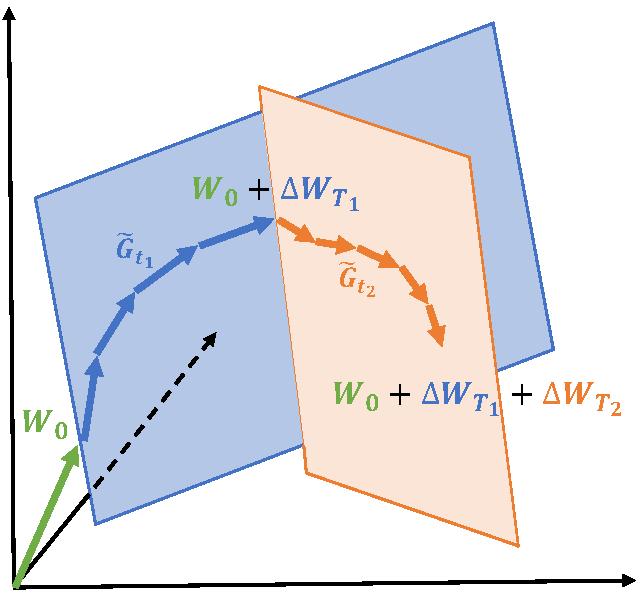
\includegraphics[width=0.58\linewidth]{figures/files/subspace_learning.pdf}
    \caption{\small{ Learning through low-rank subspaces $\Delta W_{T_1}$ and $\Delta W_{T_2}$ using \lowrank{}. For $t_1 \in [0, T_1 - 1]$, $W$ are updated by projected gradients $\tilde G_{t_1}$ in a subspace determined by fixed $P_{t_1}$ and $Q_{t_1}$. After $T_1$ steps, the subspace is changed by recomputing $P_{t_2}$ and $Q_{t_2}$ for $t_2 \in [T_1, T_2 - 1]$, and the process repeats until convergence.}}
    \label{fig:subspace_learning}
\vspace{-3mm}
\end{figure}

We allow \lowrank{} to switch across low-rank subspaces:
\begin{equation}
    \label{eq:represent_low_rank_updates_multiple}
    W_t = W_0 + \Delta W_{T_1} + \Delta W_{T_2} + \ldots + \Delta W_{T_n},
\end{equation}
where $t \in \left[\sum_{i=1}^{n-1} T_i, \sum_{i=1}^{n} T_i\right]$ and $\Delta W_{T_i} = \eta\sum_{t=0}^{T_i-1} \tilde{G_t}$ is the summation of all $T_i$ updates within the $i$-th subspace.
When switching to $i$-th subspace at step $t=T_i$, we re-initialize the projector $P_t$ and $Q_t$ by performing SVD on the current gradient $G_t$ by Equation \ref{eq:svd_p_q}.
We illustrate how the trajectory of $\tilde{G_t}$ traverses through multiple low-rank subspaces in Fig.~\ref{fig:subspace_learning}.
In the experiment section, we show that allowing multiple low-rank subspaces is the key to achieving the successful pre-training of LLMs.

Following the above procedure, the switching frequency $T$ becomes a hyperparameter. The ablation study (Fig.~\ref{fig:ablation}) shows a sweet spot exists. A very frequent subspace change increases the overhead (since new $P_t$ and $Q_t$ need to be computed) and breaks the condition of constant projection in Theorem~\ref{thm:convgpg}. In practice, it may also impact the fidelity of the optimizer states, which accumulate over multiple training steps. On the other hand, a less frequent change may make the algorithm stuck into a region that is no longer important to optimize (convergence proof in Theorem~\ref{thm:convgpg} only means good progress in the designated subspace, but does not mean good overall performance). While optimal $T$ depends on the total training iterations and task complexity, we find that a value between $T=50$ to $T=1000$ makes no much difference. Thus, the total computational overhead induced by SVD is negligible ($< 10\%$) compared to other memory-efficient training techniques such as memory offloading \citep{rajbhandariZeROMemoryOptimizations2020}.

\subsection{Memory-Efficient Optimization}

\newlength\myindent
\setlength\myindent{2em}
\newcommand\bindent{%
  \begingroup
  \setlength{\itemindent}{\myindent}
  \addtolength{\algorithmicindent}{\myindent}
}
\newcommand\eindent{\endgroup}



\begin{algorithm}[tb]
   \caption{Adam with \lowrank}
   \label{alg:low_rank_adam}
 \begin{algorithmic}
   \STATE {\bfseries Input:} A layer weight matrix $W \in \mathbb{R}^{m \times n}$ with $m \leq n$. Step size $\eta$, scale factor $\alpha$, decay rates $\beta_1, \beta_2$, rank $r$, subspace change frequency $T$.
   \STATE Initialize first-order moment $M_0 \in \mathbb{R}^{n \times r} \gets 0$
   \STATE Initialize second-order moment $V_0 \in \mathbb{R}^{n \times r} \gets 0$
   \STATE Initialize step $t \gets 0$
   \REPEAT
   \STATE $G_t \in \mathbb{R}^{m \times n} \gets - \nabla_W \phi_t(W_t)$ 
   \IF{$t \bmod T = 0$}
   \STATE $U, S, V \gets \text{SVD}(G_t)$
   \STATE $P_t \gets U[:, :r]$ \hfill \COMMENT{Initialize left projector as $m \leq n$}
   \ELSE
   \STATE $P_t \gets P_{t-1}$ \hfill \COMMENT{Reuse the previous projector}
   \ENDIF
   \STATE $R_t \gets P_{t}^{\top} G_t$ \hfill \COMMENT{Project gradient into compact space}
   \\\hrulefill
   \STATE {\bfseries $\update(R_t)$ by Adam}
   \bindent
   \hspace{\algorithmicindent} \STATE $M_t \gets \beta_1 \cdot M_{t-1} + (1 - \beta_1) \cdot R_t$ 
   \hspace{\algorithmicindent} \STATE $V_t \gets \beta_2 \cdot V_{t-1} + (1 - \beta_2) \cdot R_t^2$ 
   \hspace{\algorithmicindent} \STATE $M_t \gets M_t / (1 - \beta_1^t)$
   \hspace{\algorithmicindent} \STATE $V_t \gets V_t / (1 - \beta_2^t)$ 
   \hspace{\algorithmicindent} \STATE $N_t \gets M_t / (\sqrt{V_t} + \epsilon)$
   \eindent
   \\\hrulefill
   \STATE $\tilde G_t \gets \alpha \cdot P N_t$ \hfill \COMMENT{Project back to original space}
   \STATE $W_t \gets W_{t-1} + \eta \cdot \tilde G_t$
   \STATE $t \gets t + 1$
   \UNTIL{convergence criteria met}
   \RETURN $W_t$
 \end{algorithmic}
\end{algorithm}


\textbf{Reducing memory footprint of gradient statistics.} \lowrank{} significantly reduces the memory cost of optimizer that heavily rely on component-wise gradient statistics, such as Adam \citep{kingmaAdamMethodStochastic2014}. 
When $\rho_t \equiv \mathrm{Adam}$, by projecting $G_t$ into its low-rank form $R_t$, Adam's gradient regularizer $\rho_t(R_t)$ only needs to track low-rank gradient statistics.
where $M_t$ and $V_t$ are the first-order and second-order momentum, respectively. 
\lowrank{} computes the low-rank normalized gradient $N_t$ as follows:
\begin{equation}
    \label{eq:low_rank_normalized_gradient}
    N_t = \rho_t(R_t) = M_t / (\sqrt{V_t} + \epsilon).
\end{equation}
\lowrank{} can also apply to other optimizers (e.g., Adafactor) that have similar update rules and require a large amount of memory to store gradient statistics. 
\paragraph{Reducing memory usage of projection matrices.} To achieve the best memory-performance trade-off, we only use one project matrix $P$ or $Q$, projecting the gradient $G$ into $P^\top G$ if $m \leq n$ and $G Q$ otherwise. We present the algorithm applying \lowrank{} to Adam in Algorithm~\ref{alg:low_rank_adam}. 

With this setting, \lowrank{} requires less memory than LoRA during training.
As \lowrank{} can always merge $\Delta W_t$ to $W_0$ during weight updates, it does not need to store a separate low-rank factorization $BA$.
In total, \lowrank{} requires $(mn + mr + 2nr)$ memory, while LoRA requires $(mn + 3mr + 3nr)$ memory.
A comparison between \lowrank{} and LoRA is shown in Table~\ref{tab:lora_compare}.

As Theorem \ref{thm:convgpg} does not require the projection matrix to be carefully calibrated, we can further reduce the memory cost of projection matrices by quantization and efficient parameterization, which we leave for future work.

\subsection{Combining with Existing Techniques}

\lowrank{} is compatible with existing memory-efficient optimization techniques.
In our work, we mainly consider applying \lowrank{} with 8-bit optimizers and per-layer weight updates.

\paragraph{8-bit optimizers.}
\citet{dettmers8bitOptimizersBlockwise2021} proposed 8-bit Adam optimizer that maintains 32-bit optimizer performance at a fraction of the memory footprint.
We apply \lowrank{} directly to the existing implementation of 8-bit Adam.

\paragraph{Per-layer weight updates.}
In practice, the optimizer typically performs a single weight update for all layers after backpropagation. This is done by storing the entire weight gradients in memory. 
To further reduce the memory footprint during training, we adopt per-layer weight updates to \lowrank, which performs the weight updates during backpropagation. This is the same technique proposed in recent works to reduce memory requirement \citep{lvAdaLomoLowmemoryOptimization2023,lvFullParameterFinetuning2023}.



\subsection{Hyperparameters of \lowrank{}}
\label{sec:lowrank-hyperparams}


In addition to Adam's original hyperparameters, \lowrank{} only introduces very few additional hyperparameters: the rank $r$ which is also present in LoRA, the subspace change frequency $T$ (see Sec.~\ref{sec:composition-subspace}), and the scale factor $\alpha$. 

Scale factor $\alpha$ controls the strength of the low-rank update, which is similar to the scale factor $\alpha/r$ appended to the low-rank adaptor in \citet{huLoRALowRankAdaptation2021}.
We note that the $\alpha$ does not depend on the rank $r$ in our case. 
This is because, when $r$ is small during pre-training, $\alpha/r$ significantly affects the convergence rate, unlike fine-tuning.




\begin{table}[t]
    \caption{\small{Comparison between \lowrank{} and LoRA. Assume $W \in \mathbb{R}^{m \times n}$ ($m \leq n$), rank $r$.}}
    
    \label{tab:lora_compare}
    \begin{center}
    \begin{small}
    \begin{tabular}{lcc}
    \toprule
               & \lowrank{} & LoRA \\
    \midrule
    Weights          & $mn$   & $mn+mr+nr$ \\
    Optim States           & $mr + 2nr$   & $2mr + 2nr$  \\
    \midrule
    Multi-Subspace   & \cmark   & \xmark \\
    Pre-Training   & \cmark   & \xmark \\
    Fine-Tuning   & \cmark   & \cmark \\
    \bottomrule
    \end{tabular}
    \end{small}
    \end{center}
\vspace{-6mm}
\end{table}


\subsection{Introduction}

Natural gradient methods are optimization algorithms that adjust parameter updates according to the geometry of the parameter space, leading to faster convergence compared to standard gradient descent. They precondition the gradient using the inverse of the Fisher Information Matrix (FIM). However, computing and storing the full FIM and its inverse is computationally infeasible for large-scale models due to their high dimensionality.

To address this challenge, we propose an \textbf{online natural gradient algorithm} that operates in a low-rank subspace of the gradient space. By projecting gradients onto this subspace and approximating the FIM within it, we can efficiently compute natural gradient updates without explicit layer-wise information.

\subsection{Algorithm Description}

The algorithm consists of the following key steps:

\begin{enumerate}
    \item \textbf{Low-Rank Gradient Projection}
    \item \textbf{Gradient History Buffer Maintenance}
    \item \textbf{FIM Approximation Using Gradient History}
    \item \textbf{Natural Gradient Computation via Woodbury Identity}
    \item \textbf{Efficient Computation Using Cholesky Decomposition}
\end{enumerate}

We will explain each step in detail.

\subsubsection{Step 1: Low-Rank Gradient Projection}

Given a full-rank gradient tensor $\boldsymbol{g} \in \mathbb{R}^{n_1 \times n_2 \times \cdots \times n_d}$, we project it onto a low-rank subspace using Tucker decomposition. The Tucker decomposition approximates $\boldsymbol{g}$ as:

\[
\boldsymbol{g} \approx \mathcal{G} = \mathcal{C} \times_1 \mathbf{U}^{(1)} \times_2 \mathbf{U}^{(2)} \times_3 \cdots \times_d \mathbf{U}^{(d)},
\]

where:

\begin{itemize}
    \item $\mathcal{C} \in \mathbb{R}^{r_1 \times r_2 \times \cdots \times r_d}$ is the core tensor.
    \item $\mathbf{U}^{(i)} \in \mathbb{R}^{n_i \times r_i}$ are the factor matrices (orthogonal matrices).
    \item $\times_i$ denotes the mode-$i$ tensor-matrix product.
    \item $r_i$ is the rank along mode $i$, with $r_i \ll n_i$.
\end{itemize}

The low-rank representation (transformed gradient) is obtained by:

\[
\boldsymbol{g}_{\text{low}} = \text{Transform}(\boldsymbol{g}) = \boldsymbol{g} \times_1 (\mathbf{U}^{(1)})^\top \times_2 (\mathbf{U}^{(2)})^\top \times_3 \cdots \times_d (\mathbf{U}^{(d)})^\top.
\]

\subsubsection{Step 2: Gradient History Buffer Maintenance}

We maintain a buffer of the recent $s$ low-rank gradient vectors to capture local curvature information. Let $\boldsymbol{g}_t$ be the transformed low-rank gradient at iteration $t$, flattened into a vector:

\[
\boldsymbol{g}_t \in \mathbb{R}^{k}, \quad \text{where } k = r_1 r_2 \cdots r_d.
\]

We store the recent $s$ gradients in the matrix $\mathbf{G}$:

\[
\mathbf{G} = [\boldsymbol{g}_{t - s + 1}, \boldsymbol{g}_{t - s + 2}, \dots, \boldsymbol{g}_t] \in \mathbb{R}^{k \times s}.
\]

\subsubsection{Step 3: Approximating the Fisher Information Matrix}

We approximate the FIM within the low-rank subspace using the outer products of the stored gradients:

\[
\mathbf{F} = \lambda \mathbf{I}_k + \mathbf{G} \mathbf{G}^\top,
\]

where:

\begin{itemize}
    \item $\lambda > 0$ is a damping term to ensure numerical stability.
    \item $\mathbf{I}_k$ is the $k \times k$ identity matrix.
\end{itemize}

\subsubsection{Step 4: Computing the Natural Gradient via Woodbury Identity}

Directly computing $\mathbf{F}^{-1}$ is computationally expensive for large $k$. Instead, we use the \textbf{Woodbury identity} to efficiently compute $\mathbf{F}^{-1} \boldsymbol{g}_t$:

\[
\mathbf{F}^{-1} \boldsymbol{g}_t = \frac{1}{\lambda} \left( \boldsymbol{g}_t - \mathbf{G} \left( \lambda \mathbf{I}_s + \mathbf{G}^\top \mathbf{G} \right)^{-1} \mathbf{G}^\top \boldsymbol{g}_t \right).
\]

Let us define:

\begin{itemize}
    \item $\mathbf{S} = \lambda \mathbf{I}_s + \mathbf{G}^\top \mathbf{G} \in \mathbb{R}^{s \times s}$.
    \item $\boldsymbol{y} = \mathbf{G}^\top \boldsymbol{g}_t \in \mathbb{R}^s$.
\end{itemize}

Then, we compute:

\begin{enumerate}
    \item $\mathbf{S} = \lambda \mathbf{I}_s + \mathbf{G}^\top \mathbf{G}$.
    \item Solve $\mathbf{S} \boldsymbol{z} = \boldsymbol{y}$ for $\boldsymbol{z}$.
    \item Compute $\mathbf{F}^{-1} \boldsymbol{g}_t = \dfrac{1}{\lambda} \left( \boldsymbol{g}_t - \mathbf{G} \boldsymbol{z} \right)$.
\end{enumerate}

\subsubsection{Step 5: Efficient Computation Using Cholesky Decomposition}

To efficiently solve the linear system $\mathbf{S} \boldsymbol{z} = \boldsymbol{y}$, we use \textbf{Cholesky decomposition}:

\begin{enumerate}
    \item Compute the Cholesky factorization of $\mathbf{S}$:

    \[
    \mathbf{S} = \mathbf{L} \mathbf{L}^\top,
    \]

    where $\mathbf{L}$ is a lower triangular matrix.

    \item Solve for $\boldsymbol{u}$ in the forward substitution:

    \[
    \mathbf{L} \boldsymbol{u} = \boldsymbol{y}.
    \]

    \item Solve for $\boldsymbol{z}$ in the backward substitution:

    \[
    \mathbf{L}^\top \boldsymbol{z} = \boldsymbol{u}.
    \]
\end{enumerate}

\subsection{Algorithm Summary}

At each iteration $t$, the algorithm proceeds as follows:

\begin{enumerate}
    \item \textbf{Project the Full-Rank Gradient}:

    \begin{itemize}
        \item Obtain the low-rank transformed gradient $\boldsymbol{g}_t$ using the current factors $\{\mathbf{U}^{(i)}\}$.
    \end{itemize}

    \item \textbf{Update Gradient History}:

    \begin{itemize}
        \item If the history buffer is full, remove the oldest gradient.
        \item Add $\boldsymbol{g}_t$ to the history buffer $\mathbf{G}$.
    \end{itemize}

    \item \textbf{Compute Intermediate Quantities}:

    \begin{itemize}
        \item $\mathbf{S} = \lambda \mathbf{I}_s + \mathbf{G}^\top \mathbf{G}$.
        \item $\boldsymbol{y} = \mathbf{G}^\top \boldsymbol{g}_t$.
    \end{itemize}

    \item \textbf{Solve for $\boldsymbol{z}$}:

    \begin{itemize}
        \item Use Cholesky decomposition of $\mathbf{S}$ to solve $\mathbf{S} \boldsymbol{z} = \boldsymbol{y}$.
    \end{itemize}

    \item \textbf{Compute the Natural Gradient}:

    \begin{itemize}
        \item $\tilde{\boldsymbol{g}}_t = \dfrac{1}{\lambda} \left( \boldsymbol{g}_t - \mathbf{G} \boldsymbol{z} \right)$.
    \end{itemize}

    \item \textbf{Reshape and Project Back}:

    \begin{itemize}
        \item Reshape $\tilde{\boldsymbol{g}}_t$ back to the low-rank tensor shape.
        \item Optionally, project back to the full parameter space using the inverse transform.
    \end{itemize}
\end{enumerate}

\subsection{Mathematical Formulas}

\subsubsection{Low-Rank Projection}

The transformed low-rank gradient is obtained by:

\[
\boldsymbol{g}_{\text{low}} = \boldsymbol{g} \times_1 (\mathbf{U}^{(1)})^\top \times_2 (\mathbf{U}^{(2)})^\top \times_3 \cdots \times_d (\mathbf{U}^{(d)})^\top.
\]

\subsubsection{FIM Approximation}

We approximate the FIM as:

\[
\mathbf{F} = \lambda \mathbf{I}_k + \mathbf{G} \mathbf{G}^\top.
\]

\subsubsection{Natural Gradient Computation}

Compute the natural gradient using:

\[
\tilde{\boldsymbol{g}}_t = \mathbf{F}^{-1} \boldsymbol{g}_t = \dfrac{1}{\lambda} \left( \boldsymbol{g}_t - \mathbf{G} \boldsymbol{z} \right),
\]

where $\boldsymbol{z}$ solves:

\[
\left( \lambda \mathbf{I}_s + \mathbf{G}^\top \mathbf{G} \right) \boldsymbol{z} = \mathbf{G}^\top \boldsymbol{g}_t.
\]

\subsubsection{Efficient Solution via Cholesky Decomposition}

\begin{enumerate}
    \item Compute $\mathbf{L}$ such that:

    \[
    \lambda \mathbf{I}_s + \mathbf{G}^\top \mathbf{G} = \mathbf{L} \mathbf{L}^\top.
    \]

    \item Solve for $\boldsymbol{u}$:

    \[
    \mathbf{L} \boldsymbol{u} = \boldsymbol{y}.
    \]

    \item Solve for $\boldsymbol{z}$:

    \[
    \mathbf{L}^\top \boldsymbol{z} = \boldsymbol{u}.
    \]

    \item Compute the natural gradient:

    \[
    \tilde{\boldsymbol{g}}_t = \dfrac{1}{\lambda} \left( \boldsymbol{g}_t - \mathbf{G} \boldsymbol{z} \right).
    \]
\end{enumerate}

\subsection{Notes on Implementation}

\subsubsection{Avoiding Large Matrix Inversions}

By using the Woodbury identity and Cholesky decomposition, we avoid inverting large matrices of size $k \times k$, where $k$ can be very large.

\subsubsection{Computational Efficiency}

\begin{itemize}
    \item \textbf{Matrix-Vector Products}: Preferred over matrix-matrix multiplications for efficiency on GPUs.
    \item \textbf{GPU Computation}: All tensors are kept on the GPU to avoid data transfer overhead.
    \item \textbf{Efficient Linear Algebra}: Utilizing optimized GPU routines for operations like matrix multiplication and Cholesky decomposition.
\end{itemize}

\subsubsection{Memory Efficiency}

The history size $s$ is kept small (e.g., $s = 10$) to limit memory usage and computational cost.

\subsubsection{Numerical Stability}

The damping term $\lambda$ ensures that $\mathbf{S}$ is positive definite, allowing for stable Cholesky decomposition.

\subsection{Conclusion}

The proposed online natural gradient algorithm efficiently approximates the natural gradient in a low-rank subspace without requiring explicit layer-wise information. By maintaining a history of recent low-rank gradients and utilizing the Woodbury identity along with Cholesky decomposition, we can compute natural gradient updates efficiently on GPUs. This makes the method suitable for large-scale optimization problems where full natural gradient methods are computationally prohibitive.
\section{Experiments}

\begin{table*}[t]
    \centering
    \caption{\small{Comparison with low-rank algorithms on pre-training various sizes of LLaMA models on C4 dataset. Validation perplexity is reported, along with a memory estimate of the total of parameters and optimizer states based on BF16 format. The actual memory footprint of \lowrank{} is reported in Fig.~\ref{fig:memory_vs_model_size}.}}
    \label{tab:lora_compare_llama}
    \begin{tabular}{lcccc}
    \toprule
               & \textbf{60M} & \textbf{130M} & \textbf{350M} & \textbf{1B} \\
    \midrule
    Full-Rank & 34.06 (0.36G) & 25.08 (0.76G) & 18.80 (2.06G) & 15.56 (7.80G) \\
    \midrule
    \textbf{\lowrank} & \textbf{34.88} (0.24G) & \textbf{25.36} (0.52G) & \textbf{18.95} (1.22G) & \textbf{15.64} (4.38G) \\
    Low-Rank & 78.18 (0.26G) & 45.51 (0.54G) & 37.41 (1.08G) & 142.53 (3.57G) \\
    LoRA & 34.99 (0.36G) & 33.92 (0.80G) & 25.58 (1.76G) & 19.21 (6.17G) \\
    ReLoRA & 37.04 (0.36G) & 29.37 (0.80G) & 29.08 (1.76G) & 18.33 (6.17G) \\
    \bottomrule
    $r / d_{model}$ & 128 / 256 & 256 / 768 & 256 / 1024 & 512 / 2048 \\
    Training Tokens & 1.1B & 2.2B & 6.4B & 13.1B \\ %
    \bottomrule
    \end{tabular}
\end{table*}











We evaluate \lowrank{} on both pre-training and fine-tuning of LLMs. All experiments run on NVIDIA A100 GPUs.\vspace{-2mm}

\begin{table}[t]
    \caption{\small{Pre-training LLaMA 7B on C4 dataset for 150K steps. Validation perplexity and memory estimate are reported.}}
    \label{tab:7b_eval}
    \centering
    \begin{tabular}{l|c|cccc}
    \toprule
    & \textbf{Mem}        & \textbf{40K} & \textbf{80K} & \textbf{120K} & \textbf{150K} \\
    \midrule
    \textbf{8-bit \lowrank{}} & 18G & 17.94 & 15.39 & 14.95 & 14.65 \\
    8-bit Adam & 26G & 18.09 & 15.47 & 14.83 & 14.61 \\
    \midrule
    Tokens (B) & & 5.2 & 10.5 & 15.7 & 19.7 \\
    \bottomrule
    \end{tabular}
    \vskip -5mm
\end{table}

 

\begin{figure*}[ht]
    \vspace{-3mm}
    \centering
    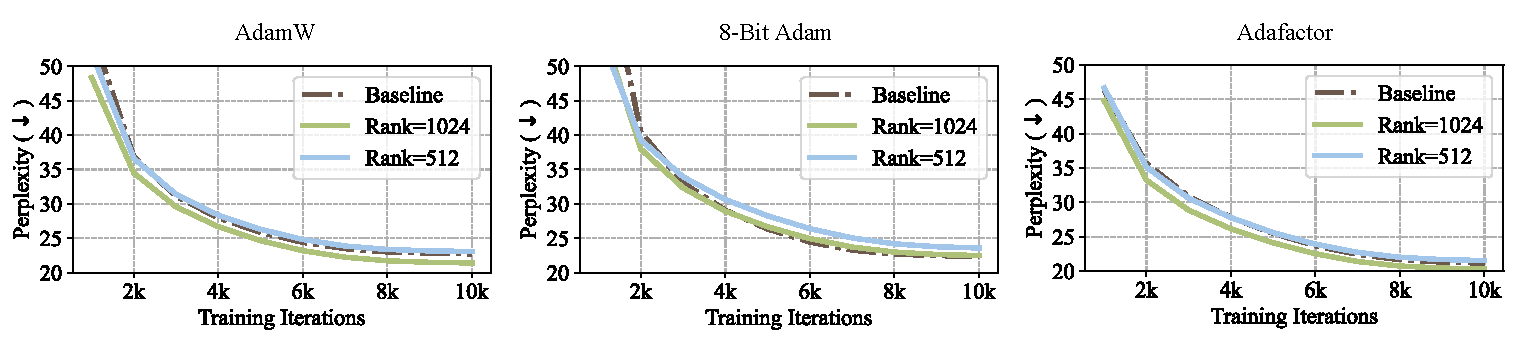
\includegraphics[width=\linewidth]{figures/train_curve.pdf}
    \vspace{-7mm}
    \caption{\small{Applying \lowrank{} to different optimizers for pre-training LLaMA 1B on C4 dataset for 10K steps. Validation perplexity over training steps is reported. We apply \lowrank{} to each optimizer with the rank of 512 and 1024, where the 1B model dimension is 2048. }}
    \vspace{-3mm}
    \label{fig:compare_optimizer}
\end{figure*}

\paragraph{Pre-training on C4.}
To evaluate its performance, we apply \lowrank{} to train LLaMA-based large language models on the C4 dataset. 
C4 dataset is a colossal, cleaned version of Common Crawl's web crawl corpus, which is mainly intended to pre-train language models and word representations \citep{raffelExploringLimitsTransfer2023}.
To best simulate the practical pre-training scenario, we train without data repetition over a sufficiently large amount of data, across a range of model sizes up to 7 Billion parameters.
\paragraph{Architecture and hyperparameters.}
We follow the experiment setup from \citet{lialinReLoRAHighRankTraining2023}, which adopts a LLaMA-based\footnote[3]{LLaMA materials in our paper are subject to LLaMA community license.} architecture with RMSNorm and SwiGLU activations \citep{zhangRootMeanSquare2019,shazeerGLUVariantsImprove2020,touvronLlamaOpenFoundation2023}. 
For each model size, we use the same set of hyperparameters across methods, except the learning rate.
We run all experiments with BF16 format to reduce memory usage, and we tune the learning rate for each method under the same amount of computational budget and report the best performance.
The details of our task setups and hyperparameters are provided in the appendix.
\paragraph{Fine-tuning on GLUE tasks.}
GLUE is a benchmark for evaluating the performance of NLP models on a variety of tasks, including sentiment analysis, question answering, and textual entailment \citep{wangGLUEMultiTaskBenchmark2019}.
We use GLUE tasks to benchmark \lowrank{} against LoRA for memory-efficient fine-tuning.

\subsection{Comparison with Existing Low-Rank Methods}

We first compare \lowrank{} with existing low-rank methods using Adam optimizer across a range of model sizes.
\paragraph{Full-Rank}
Our baseline method that applies Adam optimizer with full-rank weights and optimizer states.
\paragraph{Low-Rank}
We also evaluate a traditional low-rank approach that represents the weights by learnable low-rank factorization: $W = BA$ \citep{kamalakaraExploringLowRank2022}.
\paragraph{LoRA}
\citet{huLoRALowRankAdaptation2021} proposed LoRA to fine-tune pre-trained models with low-rank adaptors: $W = W_0 + BA$, where $W_0$ is fixed initial weights and $BA$ is a learnable low-rank adaptor. In the case of pre-training, $W_0$ is the full-rank initialization matrix.
We set LoRA alpha to 32 and LoRA dropout to 0.05 as their default settings.
\paragraph{ReLoRA}
\citet{lialinReLoRAHighRankTraining2023} proposed ReLoRA, a variant of LoRA designed for pre-training, which periodically merges $BA$ into $W$, and initializes new $BA$ with a reset on optimizer states and learning rate. ReLoRA requires careful tuning of merging frequency, learning rate reset, and optimizer states reset. We evaluate ReLoRA without a full-rank training warmup for a fair comparison.


For \lowrank{}, we set subspace frequency $T$ to 200 and scale factor $\alpha$ to 0.25 across all model sizes in Table \ref{tab:lora_compare_llama}.
For each model size, we pick the same rank $r$ for all low-rank methods, and we apply them to all multi-head attention layers and feed-forward layers in the models.
We train all models using Adam optimizer with the default hyperparameters (e.g., $\beta_1=0.9$, $\beta_2=0.999$, $\epsilon=10^{-8}$).
We also estimate the memory usage based on BF16 format, including the memory for weight parameters and optimizer states.
As shown in Table~\ref{tab:lora_compare_llama}, \lowrank{} outperforms other low-rank methods and achieves comparable performance to full-rank training.
We note that for 1B model size, \lowrank{} even outperforms full-rank baseline when $r=1024$ instead of $r=512$.
Compared to LoRA and ReLoRA, \lowrank{} requires less memory for storing model parameters and optimizer states. 
A detailed training setting of each model and memory estimation for each method are in the appendix.

\subsection{\lowrank{} with Memory-Efficient Optimizers}
We demonstrate that \lowrank{} can be applied to various learning algorithms, especially memory-efficient optimizers, to further reduce the memory footprint.
We apply \lowrank{} to AdamW, 8-bit Adam, and Adafactor optimizers \citep{shazeerAdafactorAdaptiveLearning, loshchilovDecoupledWeightDecay2019,dettmers8bitOptimizersBlockwise2021}.
We consider Adafactor with first-order statistics to avoid performance degradation.

We evaluate them on LLaMA 1B architecture with 10K training steps, and we tune the learning rate for each setting and report the best performance.
As shown in Fig.~\ref{fig:compare_optimizer}, applying \lowrank{} does not significantly affect their convergence.
By using \lowrank{} with a rank of 512, the memory footprint is reduced by up to 62.5\%, on top of the memory savings from using 8-bit Adam or Adafactor optimizer.
Since 8-bit Adam requires less memory than others, we denote 8-bit \lowrank{} as \lowrank{} with 8-bit Adam, and use it as the default method for the following experiments on 7B model pre-training and memory measurement.


\subsection{Scaling up to LLaMA 7B Architecture}
Scaling ability to 7B models is a key factor for demonstrating if \lowrank is effective for practical LLM pre-training scenarios.
We evaluate \lowrank{} on an LLaMA 7B architecture with an embedding size of 4096 and total layers of 32.
We train the model for 150K steps with 19.7B tokens, using 8-node training in parallel with a total of 64 A100 GPUs.
Due to computational constraints, we compare 8-bit \lowrank{} ($r=1024$) with 8-bit Adam with a single trial without tuning the hyperparameters.   
As shown in Table \ref{tab:7b_eval}, after 150K steps, 8-bit \lowrank{} achieves a perplexity of 14.65, comparable to 8-bit Adam with a perplexity of 14.61.



\begin{figure}[t!]
    \centering
    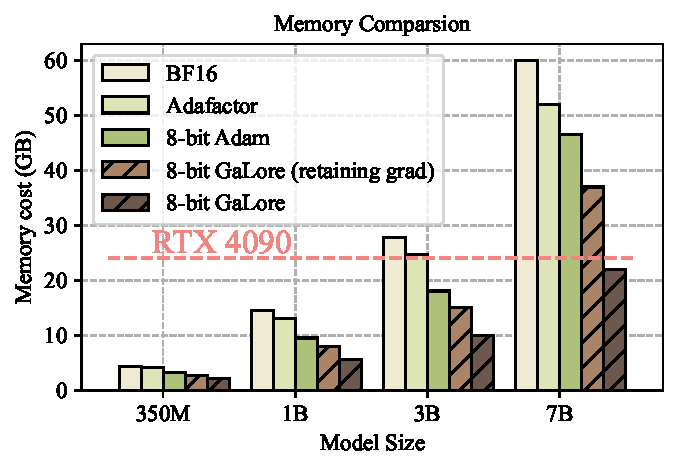
\includegraphics[width=0.9\linewidth]{figures/memory.pdf}
    \vspace{-4.5mm}
    \caption{\small{Memory usage for different methods at various model sizes, evaluated with a token batch size of 256. 8-bit \lowrank{} (retaining grad) disables per-layer weight updates but stores weight gradients during training.
    }}
    \vspace{-4mm}
    \label{fig:memory_vs_model_size}
\end{figure}


\subsection{Memory-Efficient Fine-Tuning}
\lowrank{} not only achieves memory-efficient pre-training but also can be used for memory-efficient fine-tuning.
We fine-tune pre-trained RoBERTa models on GLUE tasks using \lowrank{} and compare its performance with a full fine-tuning baseline and LoRA.
We use hyperparameters from \citet{huLoRALowRankAdaptation2021} for LoRA and tune the learning rate and scale factor for \lowrank{}.
As shown in Table~\ref{tab:fine_tuning}, \lowrank{} achieves better performance than LoRA on most tasks with less memory footprint.
This demonstrates that \lowrank{} can serve as a full-stack memory-efficient training strategy for both LLM pre-training and fine-tuning.

\begin{table}[t]
    \caption{\small Evaluating \lowrank{} for memory-efficient fine-tuning on GLUE benchmark using pre-trained RoBERTa-Base. We report the average score of all tasks.}
    \label{tab:fine_tuning}
    \centering
    \resizebox{\linewidth}{!}{%
    \begin{tabular}{l|c|cccccccc|c}
    \toprule
               & \textbf{Memory} & \textbf{CoLA} & \textbf{STS-B} & \textbf{MRPC} & \textbf{RTE} & \textbf{SST2} & \textbf{MNLI} & \textbf{QNLI} & \textbf{QQP} & \textbf{Avg} \\
    \midrule
    Full Fine-Tuning & 747M & 62.24 & 90.92 & 91.30 & 79.42 & 94.57 & 87.18 & 92.33 & 92.28 & 86.28 \\
    \midrule
    \textbf{\lowrank{} (rank=4)} & 253M & 60.35 & \textbf{90.73} & \textbf{92.25} & \textbf{79.42} & \textbf{94.04} & \textbf{87.00} & \textbf{92.24} & 91.06 & \textbf{85.89} \\
    LoRA (rank=4) & 257M & \textbf{61.38} & 90.57 & 91.07 & 78.70  & 92.89 & 86.82 & 92.18 & \textbf{91.29} & 85.61 \\
    \midrule
    \textbf{\lowrank{} (rank=8)} & 257M & 60.06 & \textbf{90.82} & \textbf{92.01} & \textbf{79.78} & \textbf{94.38} & \textbf{87.17} & 92.20 & 91.11 & \textbf{85.94} \\
    LoRA (rank=8) & 264M & \textbf{61.83} & 90.80 & 91.90 & 79.06  & 93.46 & 86.94 & \textbf{92.25} & \textbf{91.22} & 85.93 \\
    \bottomrule
    \end{tabular}
    }
    \vskip -0.1in
\end{table}





\subsection{Measurement of Memory and Throughput}
\label{sec:memory_measure}
While Table~\ref{tab:lora_compare_llama} gives the theoretical benefit of \lowrank{} compared to other methods in terms of memory usage, we also measure the actual memory footprint of training LLaMA models by various methods, with a token batch size of 256. 
The training is conducted on a single device setup without activation checkpointing, memory offloading, and optimizer states partitioning \citep{rajbhandariZeROMemoryOptimizations2020}.

\textbf{Training 7B models on consumer GPUs with 24G memory.} As shown in Fig.~\ref{fig:memory_vs_model_size}, 8-bit \lowrank{} requires significantly less memory than BF16 baseline and 8-bit Adam, and only requires 22.0G memory to pre-train LLaMA 7B with a small per-GPU token batch size (up to 500 tokens). This memory footprint is within 24GB VRAM capacity of a single GPU such as NVIDIA RTX 4090.
In addition, when activation checkpointing is enabled, per-GPU token batch size can be increased up to 4096. While the batch size is small per GPU, it can be scaled up with data parallelism, which requires much lower bandwidth for inter-GPU communication, compared to model parallelism. Therefore, it is possible that \lowrank{} can be used for elastic training~\cite{linDynamicMinibatchSGD2019} 7B models on consumer GPUs such as RTX 4090s. %

Specifically, we present the memory breakdown in Fig.~\ref{fig:memory_breakdown}.
It shows that 8-bit \lowrank{} reduces 37.92G (63.3\%) and 24.5G (52.3\%) total memory compared to BF16 Adam baseline and 8-bit Adam, respectively.
Compared to 8-bit Adam, 8-bit \lowrank{} mainly reduces the memory in two parts: (1) low-rank gradient projection reduces 9.6G (65.5\%) memory of storing optimizer states, and (2) using per-layer weight updates reduces 13.5G memory of storing weight gradients.

\textbf{Throughput overhead of \lowrank{}.} We also measure the throughput of the pre-training LLaMA 1B model with 8-bit \lowrank{} and other methods, where the results can be found in the appendix.
Particularly, the current implementation of 8-bit \lowrank{} achieves 1019.63 tokens/second, which induces 17\% overhead compared to 8-bit Adam implementation. 
Disabling per-layer weight updates for \lowrank{} achieves 1109.38 tokens/second, improving the throughput by 8.8\%. We note that our results do not require offloading strategies or checkpointing, which can significantly impact training throughput. 
We leave optimizing the efficiency of \lowrank{} implementation for future work.





\vspace{-2mm}
\section{Ablation Study}
\paragraph{How many subspaces are needed during pre-training?}

We observe that both too frequent and too slow changes of subspaces hurt the convergence, as shown in Fig.~\ref{fig:ablation} (left). The reason has been discussed in Sec.~\ref{sec:composition-subspace}. In general, for small $r$, the subspace switching should happen more to avoid wasting optimization steps in the wrong subspace, while for large $r$ the gradient updates cover more subspaces, providing more cushion. 


\begin{figure}
    \centering
        
    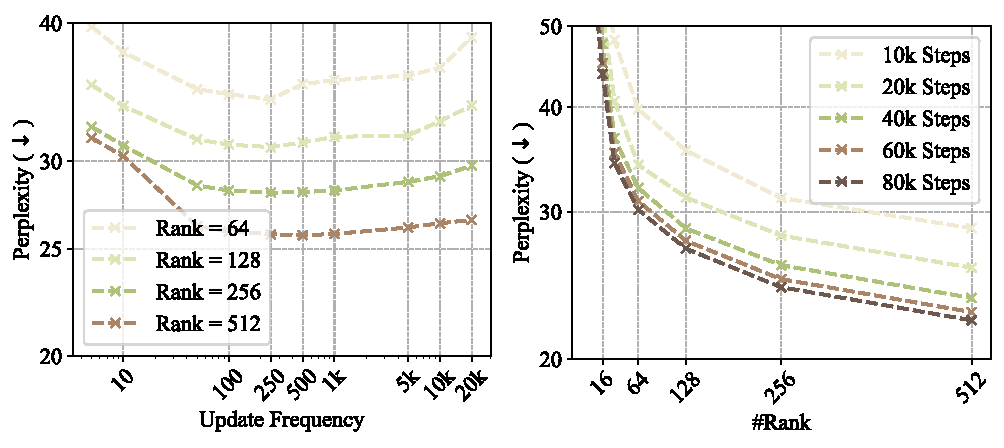
\includegraphics[width=\linewidth]{figures/files/ablation.pdf}
    \caption{\small{Ablation study of \lowrank{} on 130M models. \textbf{Left:} varying subspace update frequency $T$. \textbf{Right:} varying subspace rank and training iterations.}}
    \vspace{-7mm}
    \label{fig:ablation}
\end{figure} 


\paragraph{How does the rank of subspace affect the convergence?}
Within a certain range of rank values, decreasing the rank only slightly affects the convergence rate, causing a slowdown with a nearly linear trend.
As shown in Fig.~\ref{fig:ablation} (right), training with a rank of 128 using 80K steps achieves a lower loss than training with a rank of 512 using 20K steps.
This shows that \lowrank{} can be used to trade-off between memory and computational cost.
In a memory-constrained scenario, reducing the rank allows us to stay within the memory budget while training for more steps to preserve the performance.








\section{Conclusion}

We propose \lowrank{}, a memory-efficient pre-training and fine-tuning strategy for large language models.
\lowrank{} significantly reduces memory usage by up to 65.5\% in optimizer states while maintaining both efficiency and performance for large-scale LLM pre-training and fine-tuning.

We identify several open problems for \lowrank{}, which include (1) applying \lowrank{} on training of various models such as vision transformers \citep{dosovitskiy2021an} and diffusion models \citep{ho2020denoising}, (2) further enhancing memory efficiency by employing low-memory projection matrices, and (3) exploring the feasibility of elastic data distributed training on low-bandwidth consumer-grade hardware.

We hope that our work will inspire future research on memory-efficient training from the perspective of gradient low-rank projection. 
We believe that \lowrank{} will be a valuable tool for the community, enabling the training of large-scale models on consumer-grade hardware with limited resources.

\section*{Impact Statement}

This paper aims to improve the memory efficiency of training LLMs in order to reduce the environmental impact of LLM pre-training and fine-tuning. By enabling the training of larger models on hardware with lower memory, our approach helps to minimize energy consumption and carbon footprint associated with training LLMs.
\section*{Acknowledgments}

We thank Meta AI for computational
support. 
We appreciate the helpful feedback and discussion from Florian Sch{\"a}fer, Jeremy Bernstein, and Vladislav Lialin.
B. Chen greatly appreciates the support by Moffett AI.
Z. Wang is in part supported by NSF Awards 2145346 (CAREER), 02133861 (DMS), 2113904 (CCSS), and the NSF AI Institute for Foundations of Machine Learning (IFML).
A. Anandkumar is supported by the Bren Foundation and the Schmidt Sciences through AI 2050 senior fellow program.

\bibliography{iclr_template/iclr2025_conference}
\bibliographystyle{iclr_template/iclr2025_conference}

\end{document}
